% TODO: Update this for proper formatting:
%\documentclass[12pt,times]{article}
\documentclass[12pt]{article} % \usepackage{times}
%\usepackage[a4paper, showframe, tmargin=25mm, lmargin=25mm, rmargin=25mm, bmargin=20mm]{geometry}
\usepackage[a4paper, tmargin=25mm, lmargin=20mm, rmargin=20mm, bmargin=20mm]{geometry}
\usepackage{amsmath,amssymb,amsthm}
\usepackage{color}
\usepackage{hyperref}
\usepackage{graphicx}
\usepackage{stmaryrd}
\usepackage{listings}
\usepackage{color}
\usepackage{wrapfig}
\usepackage{url}
\usepackage{fancyvrb}
\usepackage{placeins}
\usepackage{bold-extra}
\usepackage[nounderscore]{syntax}
\usepackage{mathtools}
\usepackage{caption}
\usepackage{float}

%\usepackage{fancyhdr}
%\pagestyle{fancy}
%\rhead{Version: \GUIDEVERSION} 
%\lhead{\GUIDETITLE}
%\cfoot{}
%\thispagestyle{fancy}
% \thispagestyle{headings}

\makeatletter
\renewcommand{\maketitle}{\bgroup\setlength{\parindent}{0pt}
  \thispagestyle{empty}
  \begin{flushleft}
    \textbf{\@title}

    \vspace{3cm}
    
    \@author
    
    \begin{center}
      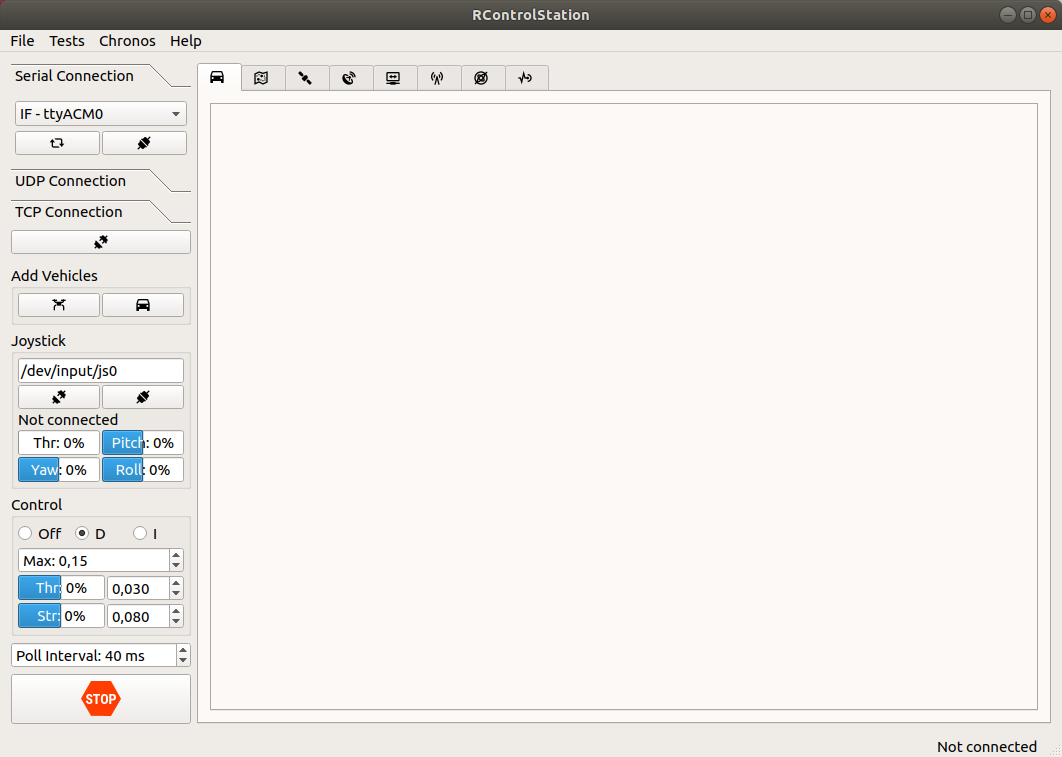
\includegraphics[width=0.7\textwidth]{./screens/RControlStation1.png}
    \end{center}
      
  \end{flushleft}\egroup
}
\makeatother


\newcommand{\GUIDEVERSION}[0]{$0.1$}
\newcommand{\GUIDETITLE}[0]{RISE Self Driving Vehicle Platform \newline \noindent
  Operator's Manual \newline \noindent Version: \GUIDEVERSION{}} 


\newenvironment{changeentry}[2]
               {
                 \noindent #1 : #2 \newline 
                 \vspace{2mm} \noindent
               }
               {
                 \vspace{2mm}
                 \hrule 
                 \vspace{2mm}
               }

\newcommand{\todo}[1]{{\color{red} \textbf{TODO:} #1}}
               


\begin{document}

\title{\GUIDETITLE}


\author{Benjamin Vedder\\ \texttt{benjamin.vedder@ri.se}\\ \vspace{5mm} Bo Joel Svensson\\ \texttt{joel.svensson@ri.se}} 

%  Use the @ symbol for simple inline code within prose:
\lstMakeShortInline[]@

\maketitle

%% \newpage

%% \section*{\small Disclaimer}

\newpage
\tableofcontents{}
\newpage


\section{Introduction}

This manual aims to outline and exemplify configuration and use of the
RISE Self Driving model Vehicle Platform (SDVP). It does not go in
depth in describing the hardware or software that runs on the
microcontrollers in for example the RC car, but rather tries to give
enough background for starting operate the system using the
RControlStation software which is a graphical user interface for
controlling and monitoring the SDVP.

RControlStation can, among much more, be used for the following:
\begin{itemize}
\item Track and trace movement of the SDVP overlaid on a map
  implemented based on OpenStreetMap.
\item Draw, load and save trajectories for the car to
  follow. Trajectories are visualised as points connected by line
  segments on the map.
\item Control the car directly via the keyboard.
\item Configure car dynamics.
\item Configure numerous parameters related to the positioning system.
\item monitor and log data obtained from the SDVP. 
\end{itemize} 

\section{RISE SDVP Hardware Overview} 

The hardware found on the RC car consists of a motor controller (the
VESC), another controller board that we call the RTK Controller and a
Raspberry Pi.  The Raspberry Pi is there to provide Wifi and/or 4G
cellular connectivity and enable for example remote debugging. The RTK
Controller implements the self driving aspects of the SDVP and
includes positioning capabilities using GPS and has two radios for
communication. The RTK Controller connects to the car steering servo,
providing its power and PWM signal for control. The RTK controller is
also connected to the VESC over CAN-bus. If a Raspberry Pi is present
in the system it is connected to the RTK Controller over USB, it is
possible to power the Pi through this connection with a modification
shown below. Some of the GPIO pins of the Pi can also be connected to
the SWD port on the RTK Controller to enable remote flashing of the
embedded software.

\vspace{5mm}

\noindent \begin{minipage}{0.33\textwidth}
  \noindent 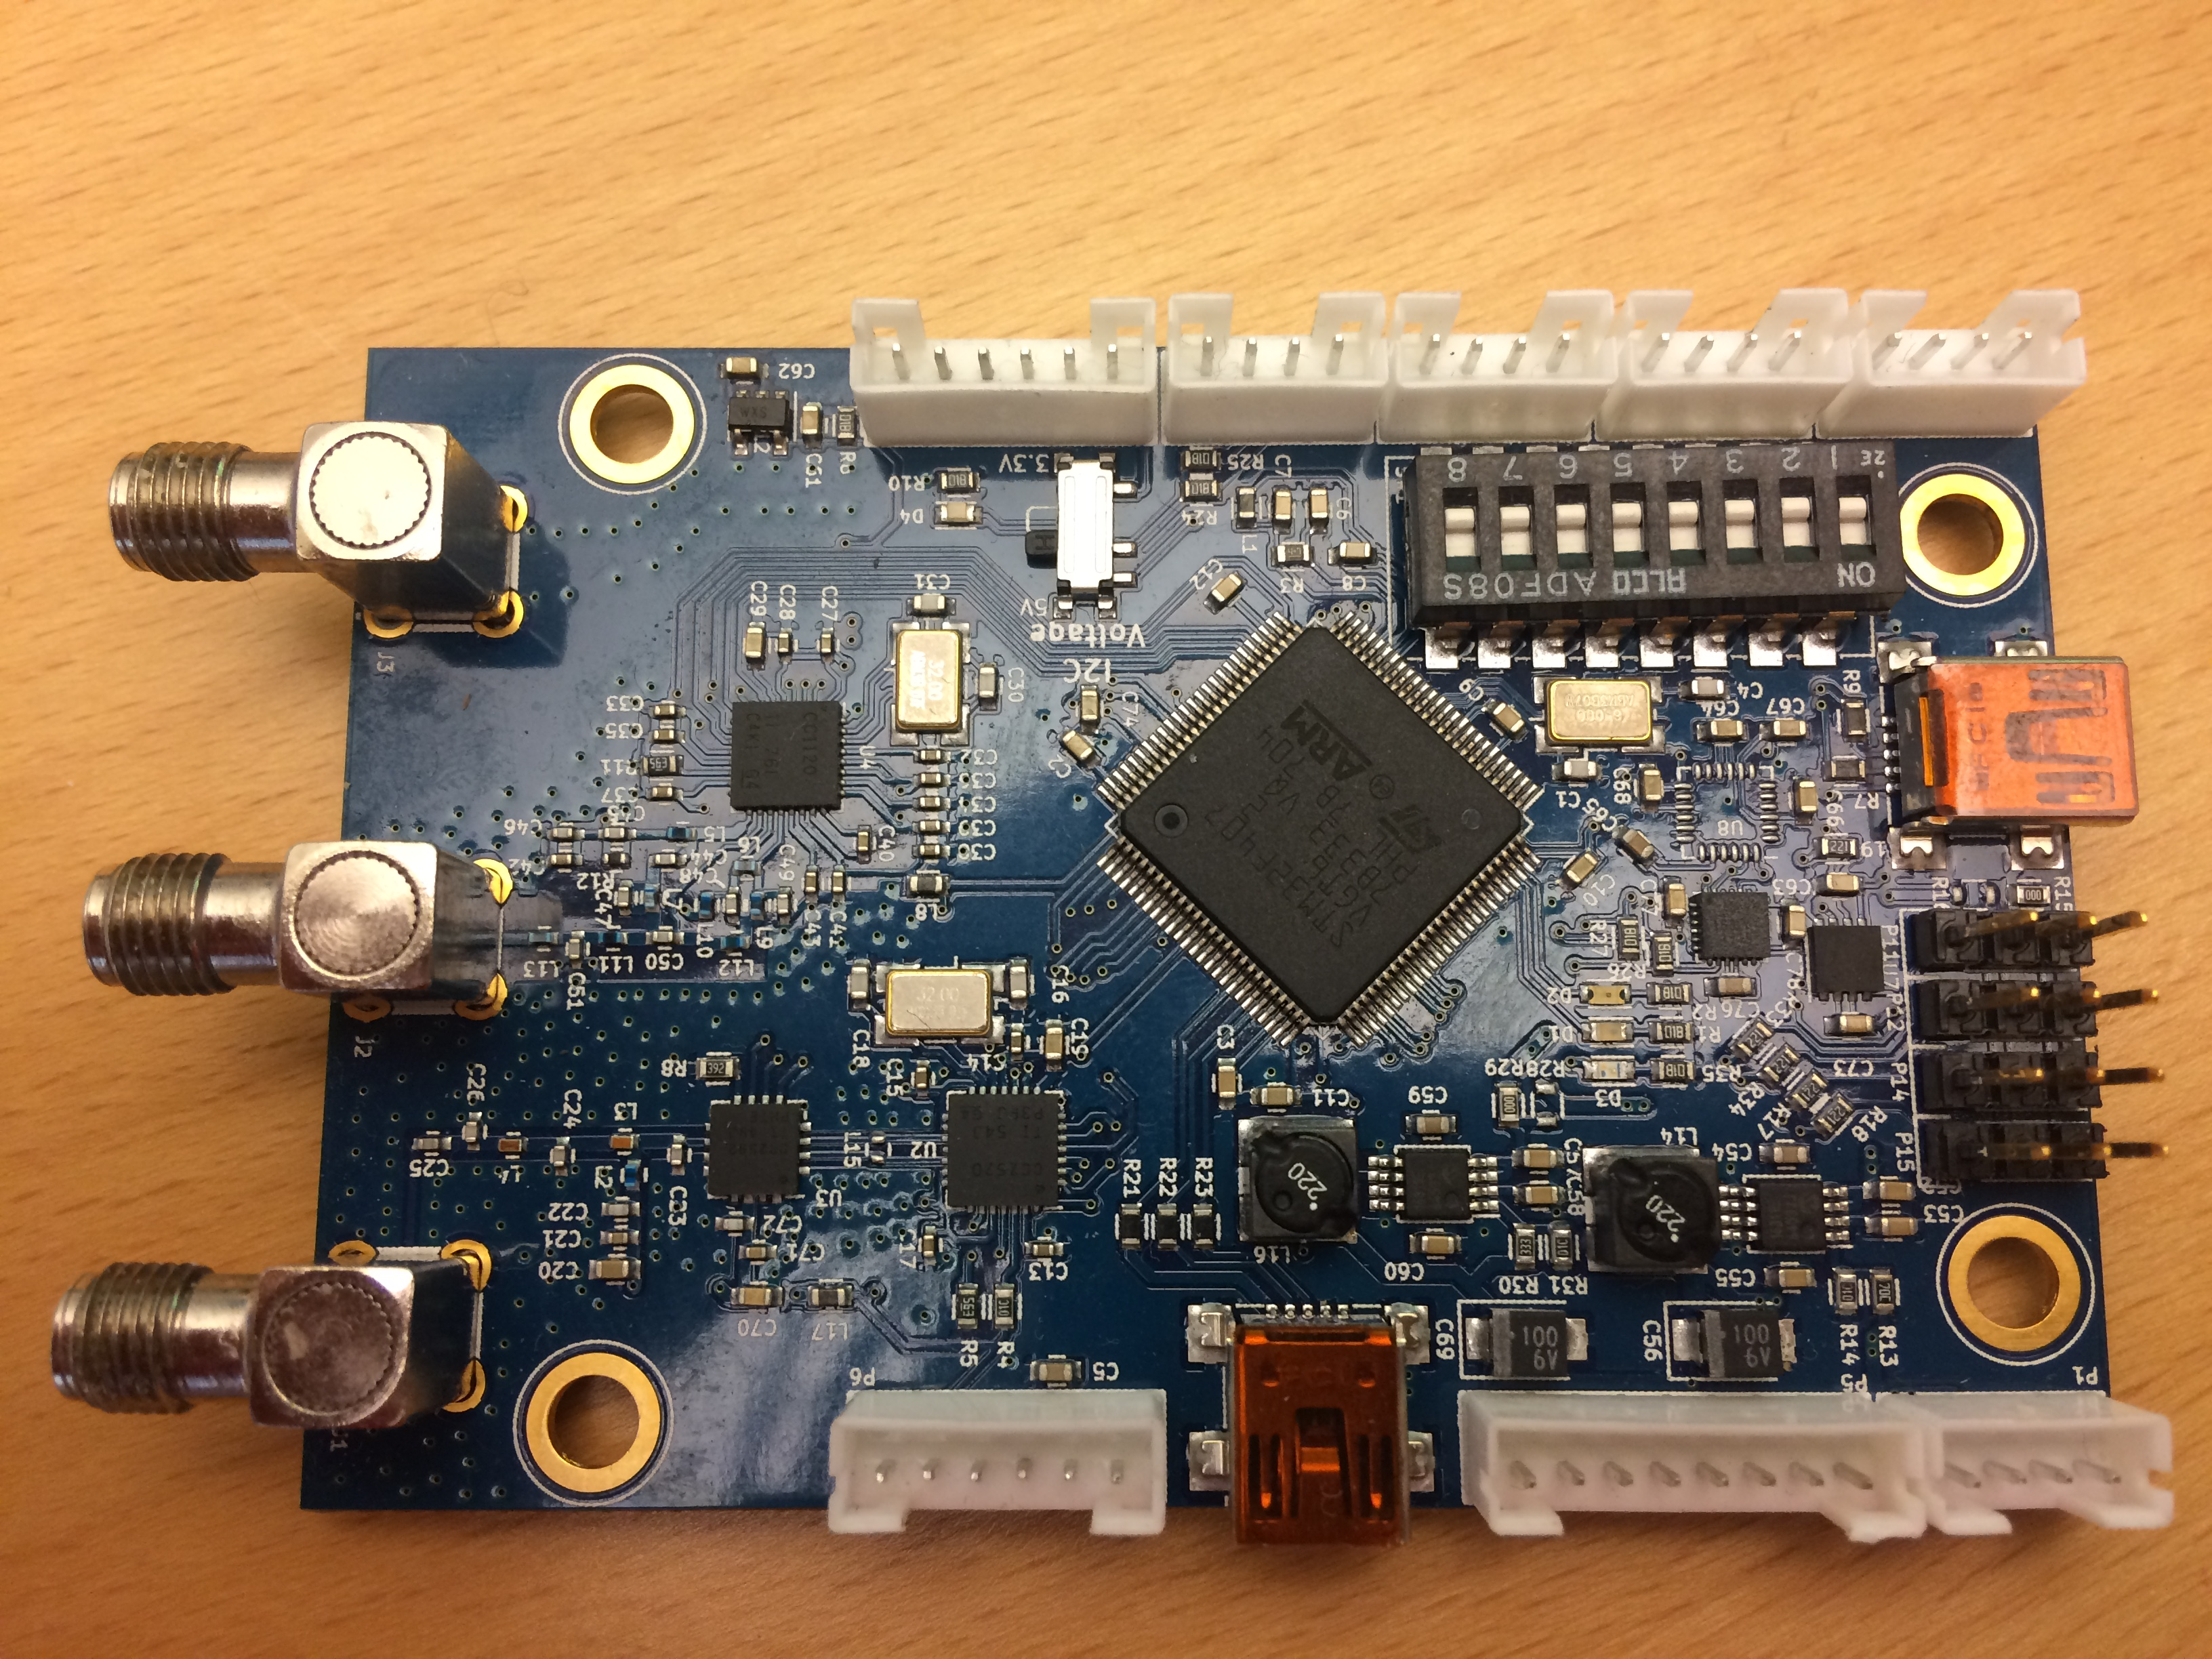
\includegraphics[width=\textwidth]{./photos/RTKControl2.JPG}
  \noindent 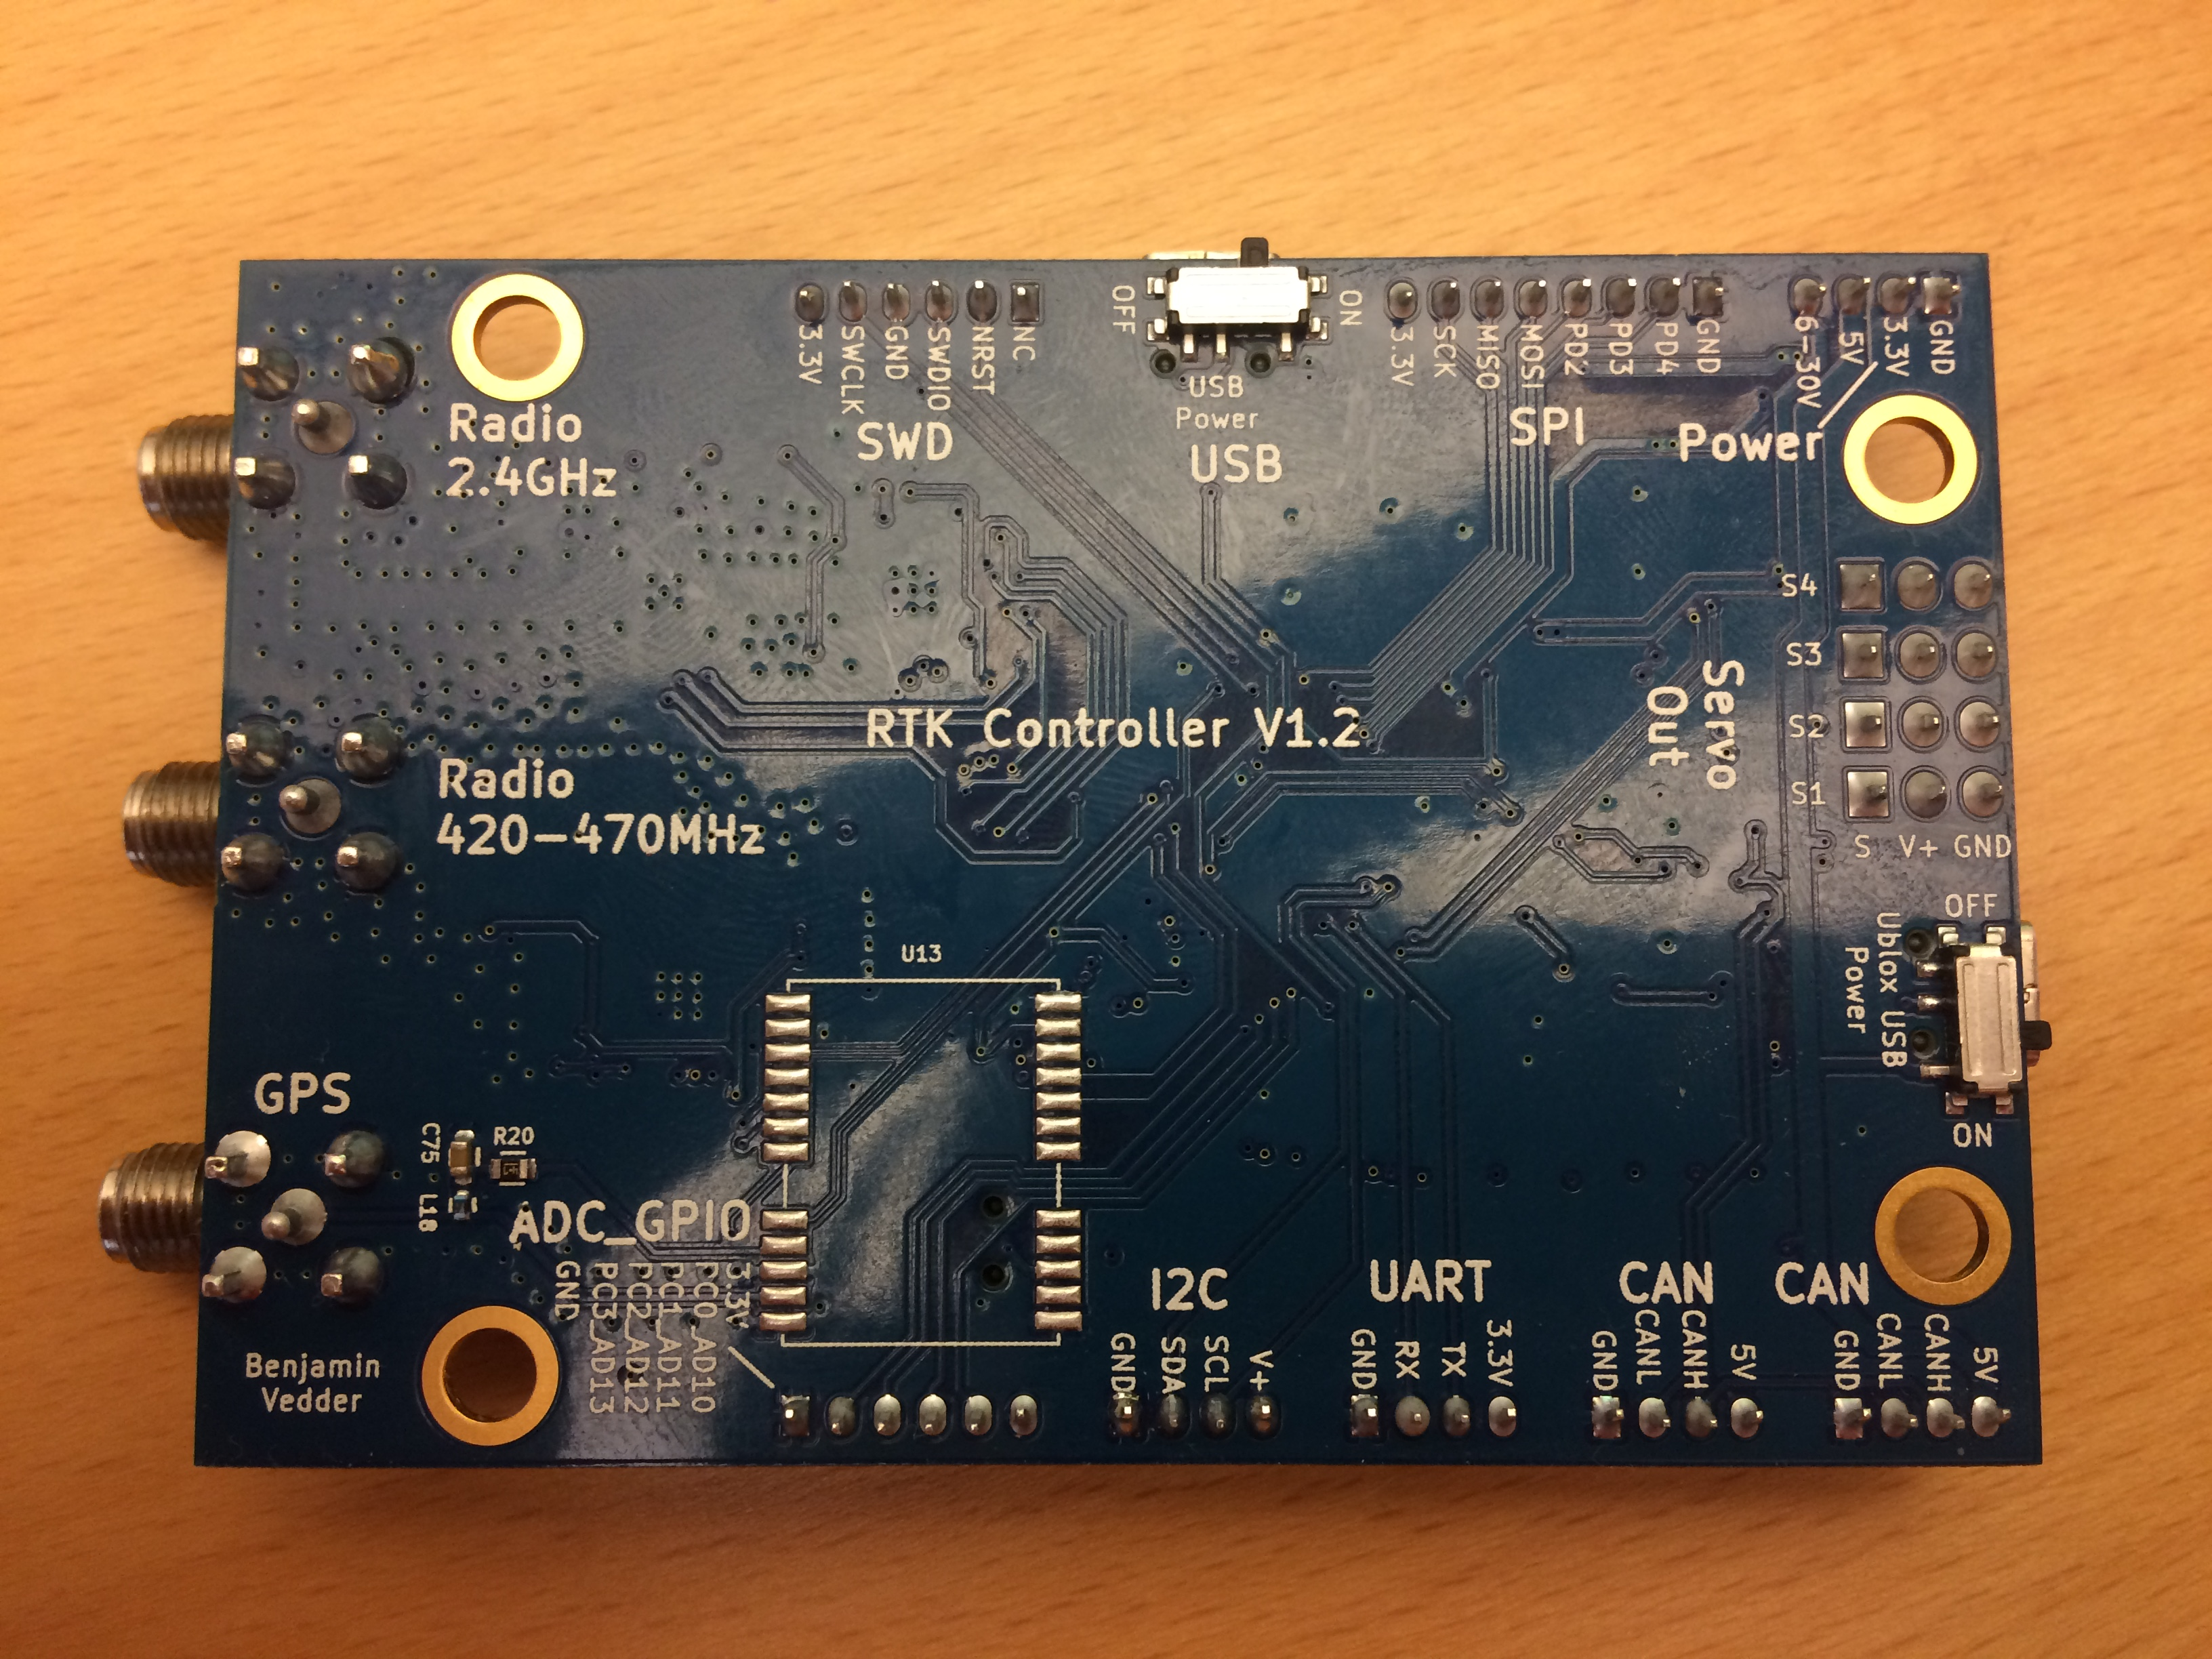
\includegraphics[width=\textwidth]{./photos/RTKControl1.JPG}
\end{minipage}
\begin{minipage}{0.66\textwidth} %% Text RTK
  The pictures show the top (top) and bottom (bottom) view of the RTK
  Controller. On the top view you can see three antenna connectors for
  GPS and radio.  There is a set of dip switches that configure the
  identity of the board. The set of connector pins along the right
  edge are for controlling servos and the write sockets are CAN, I2C,
  UART, SWD and SPI connectors.  On the bottom view you can see solder
  pads for a UBLOX chip (this card happens to not be equiped with one)
  and a small switch for toggling ``Power over USB'' to power a
  connected Raspberry Pi backwards through its USB port.  The RTK
  Controller connects to the computer running RControlStation either,
  over USB directly, over radio or over WIFI or 4G via the Raspberry
  Pi.
\end{minipage}

\vspace{5mm}

\noindent \begin{minipage}{0.66\textwidth} These pictures show the VESC
  motor controller, alone (top) and together with an RTK Controller
  and a motor (bottom). On the left side of the VESC (block of
  aluminium) you can see a battery connector.  On the other side of
  the aluminium are three cables for connecting a brushless motor.  On
  the bottom of the VESC there is also a set of connectors for CAN,
  SWD and so on. On the bottom picture, the RTK Controller is
  connected to the VESC over CAN.
  \todo{Insert information about max/min voltage} 
\end{minipage}
\begin{minipage}{0.33\textwidth} %% Text VESC
  \noindent 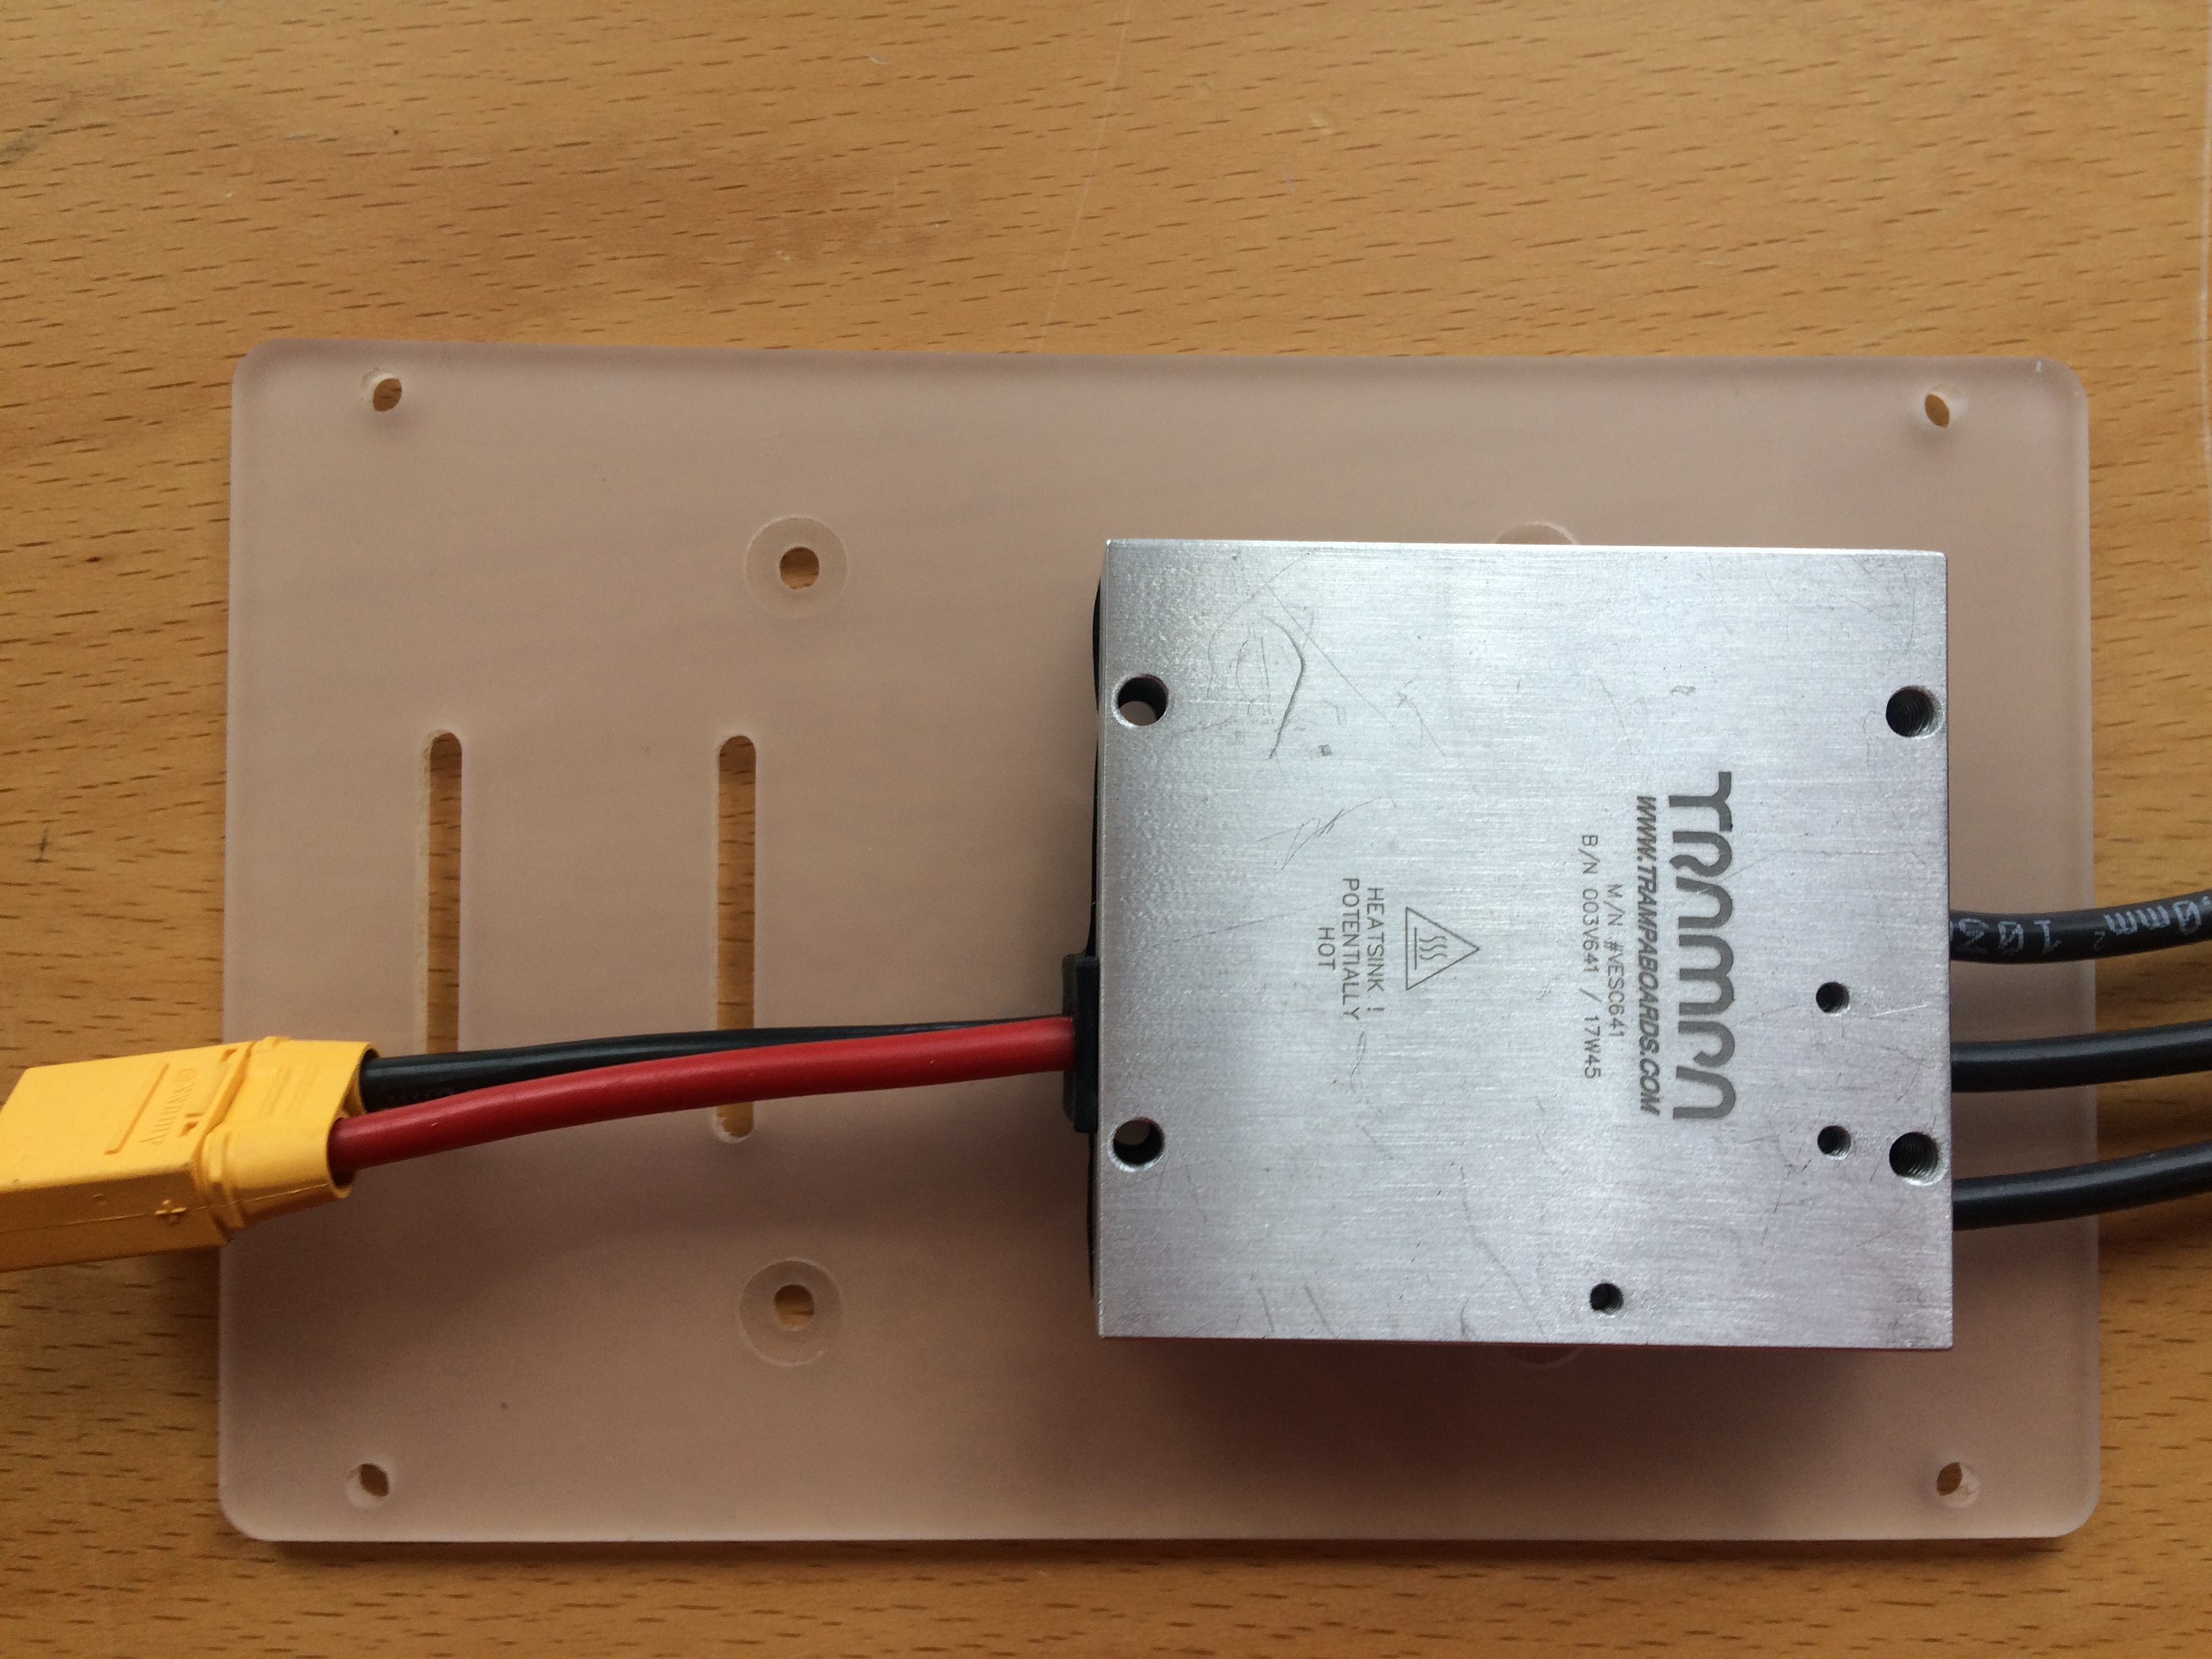
\includegraphics[width=\textwidth]{./photos/VESC.JPG}
  \noindent 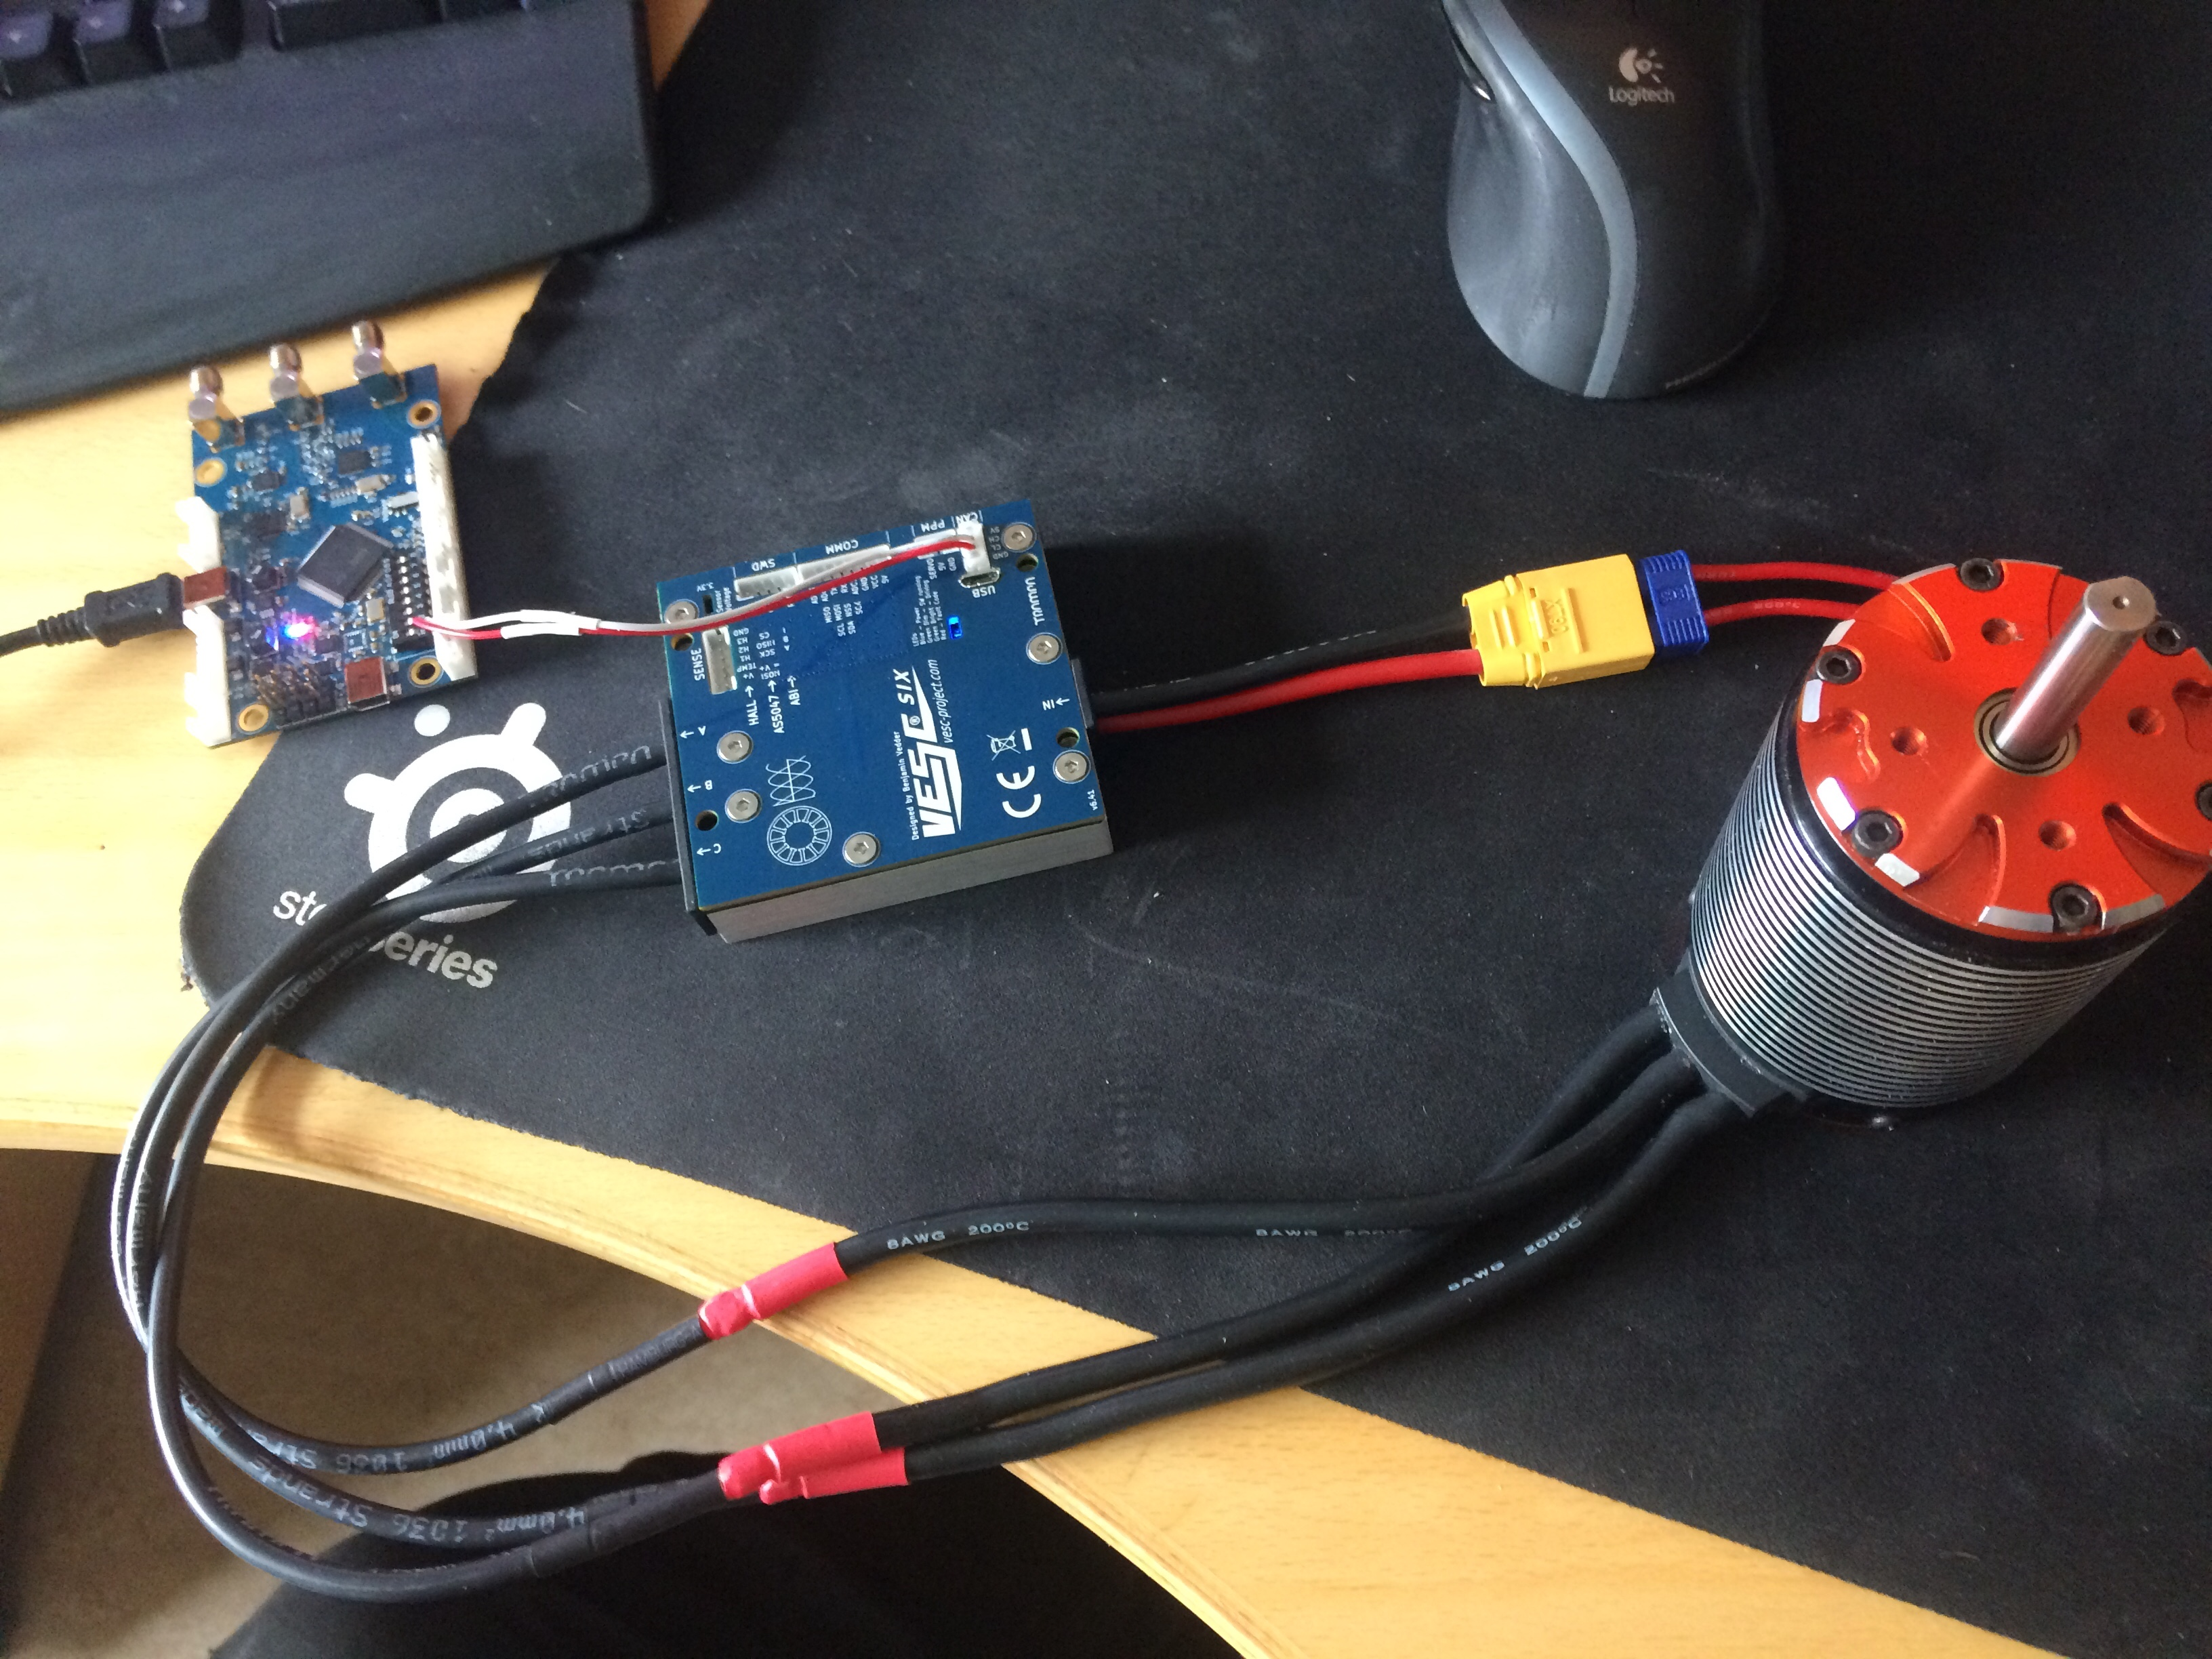
\includegraphics[width=\textwidth]{./photos/VESC_RTK.JPG}
\end{minipage}


\vspace{5mm}

\noindent \begin{minipage}{0.33\textwidth}
  \noindent 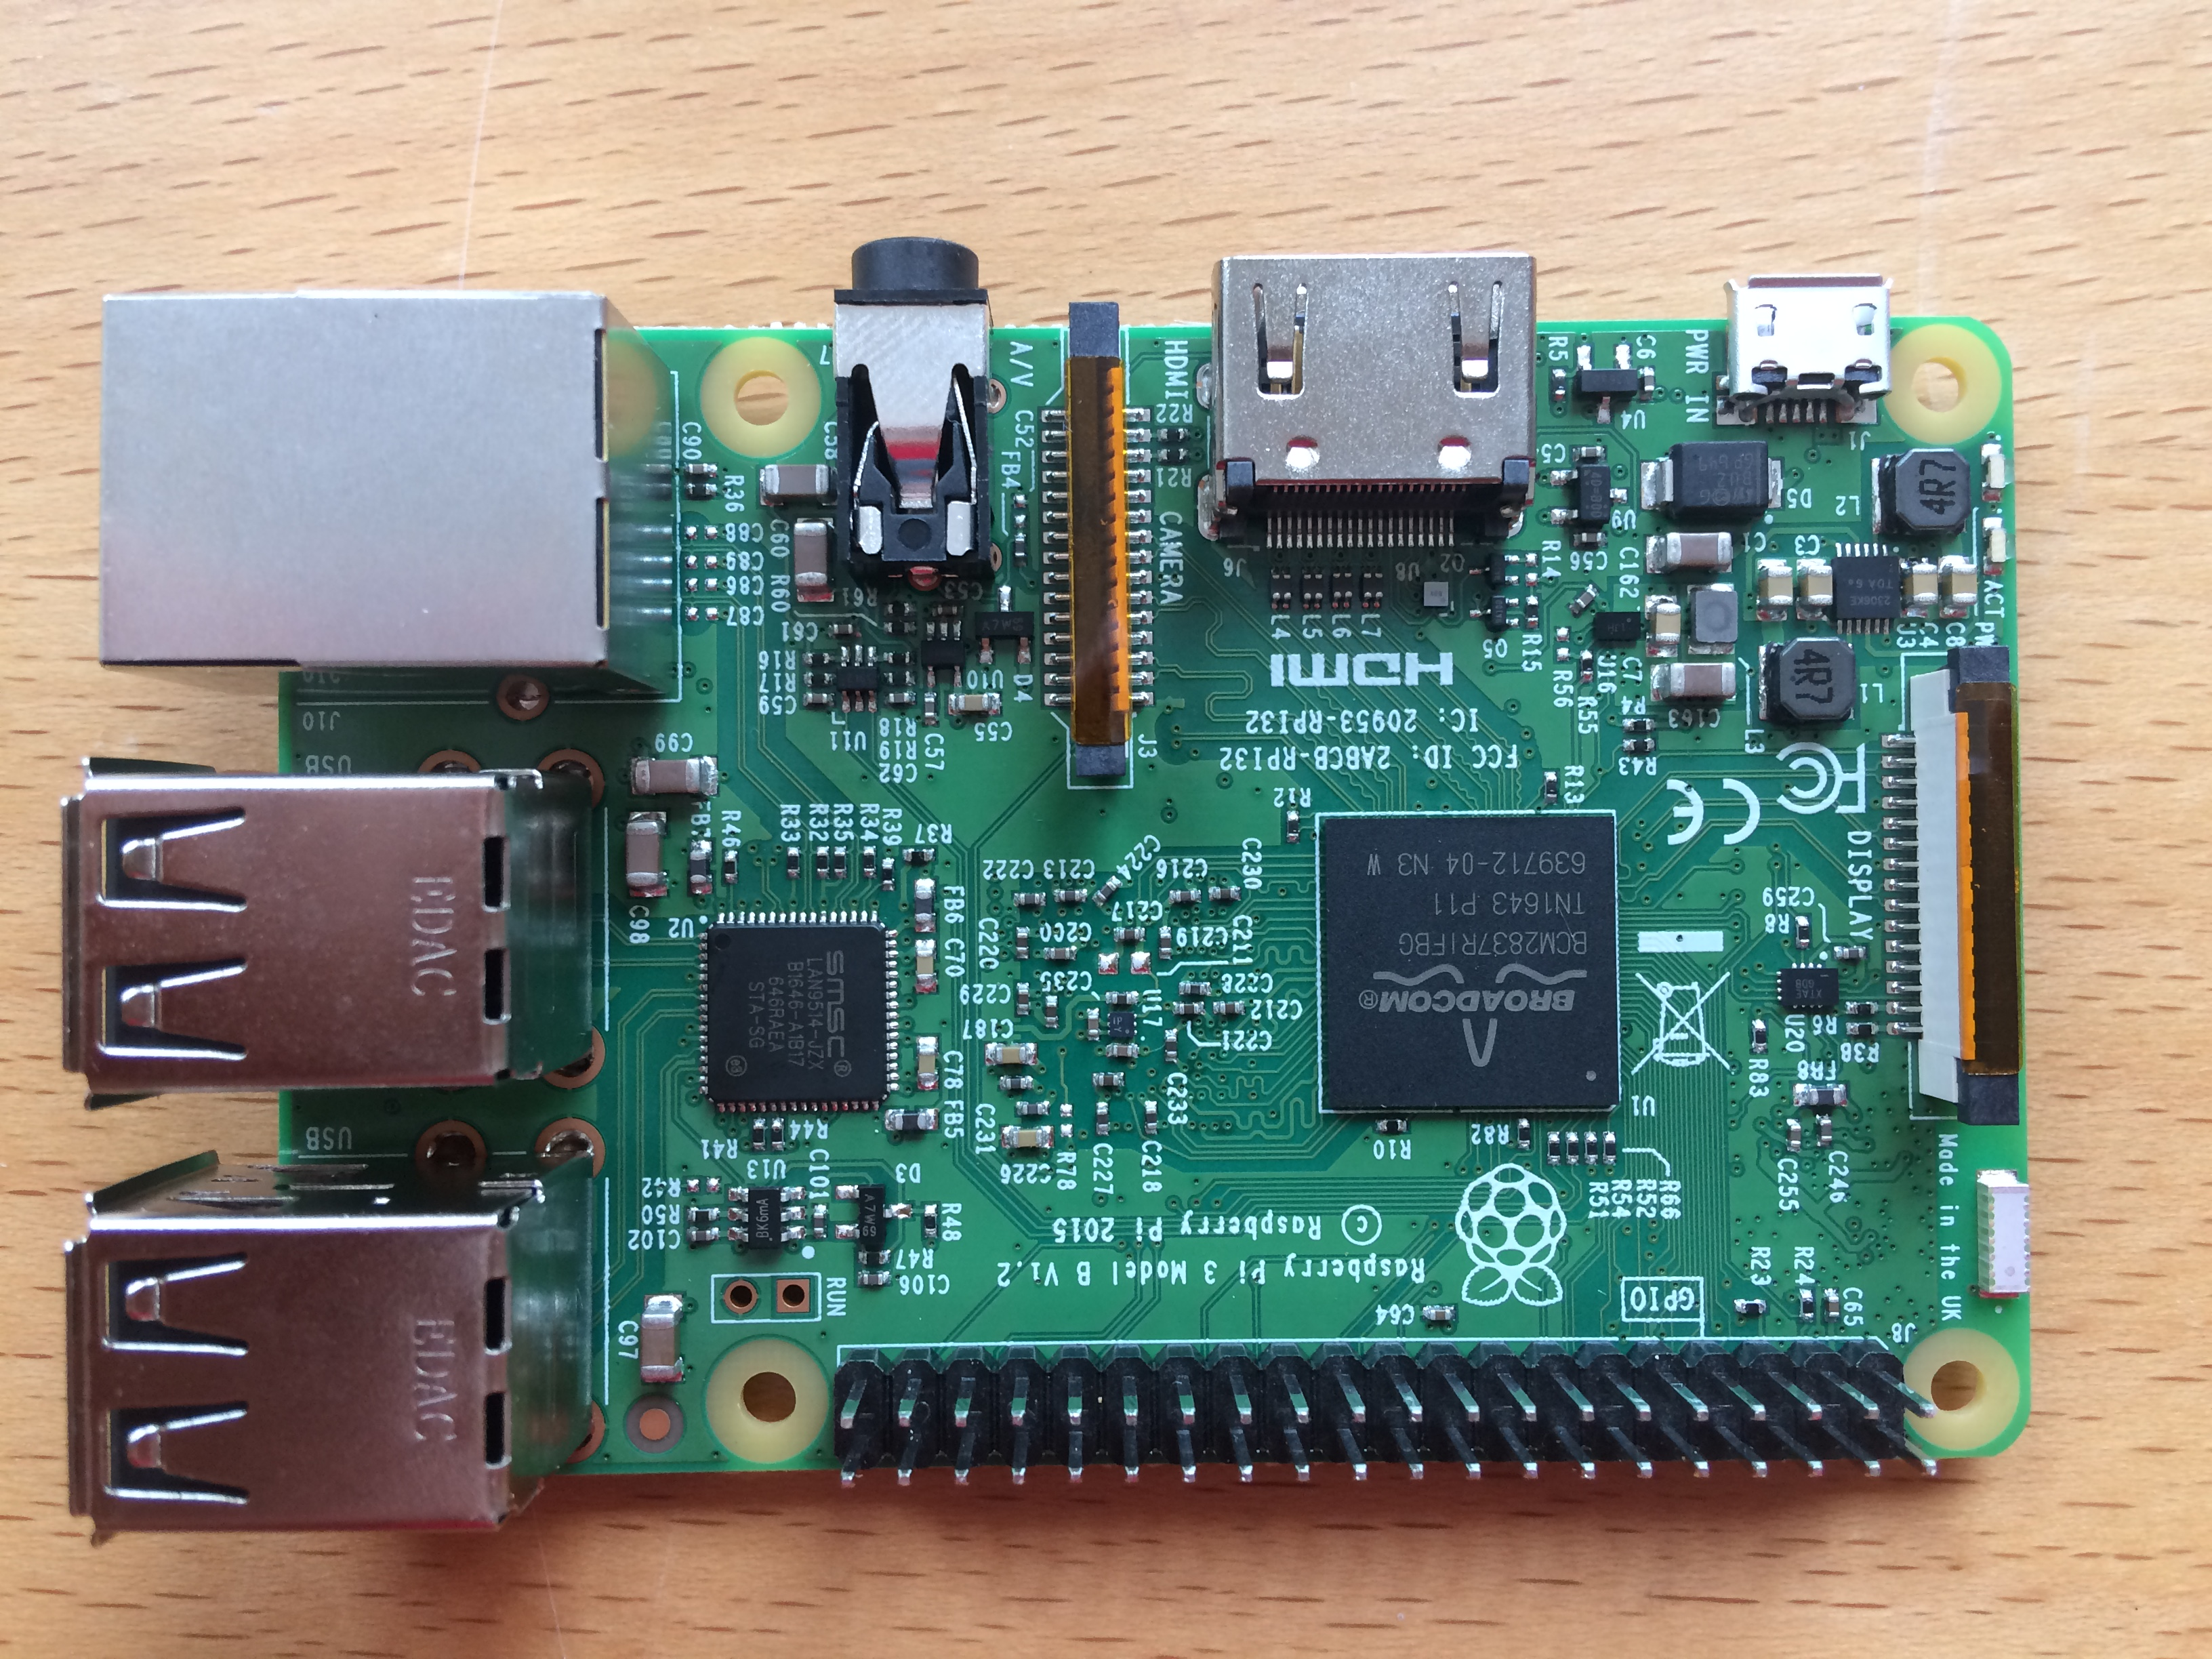
\includegraphics[width=\textwidth]{./photos/Pi1.JPG}
  \noindent 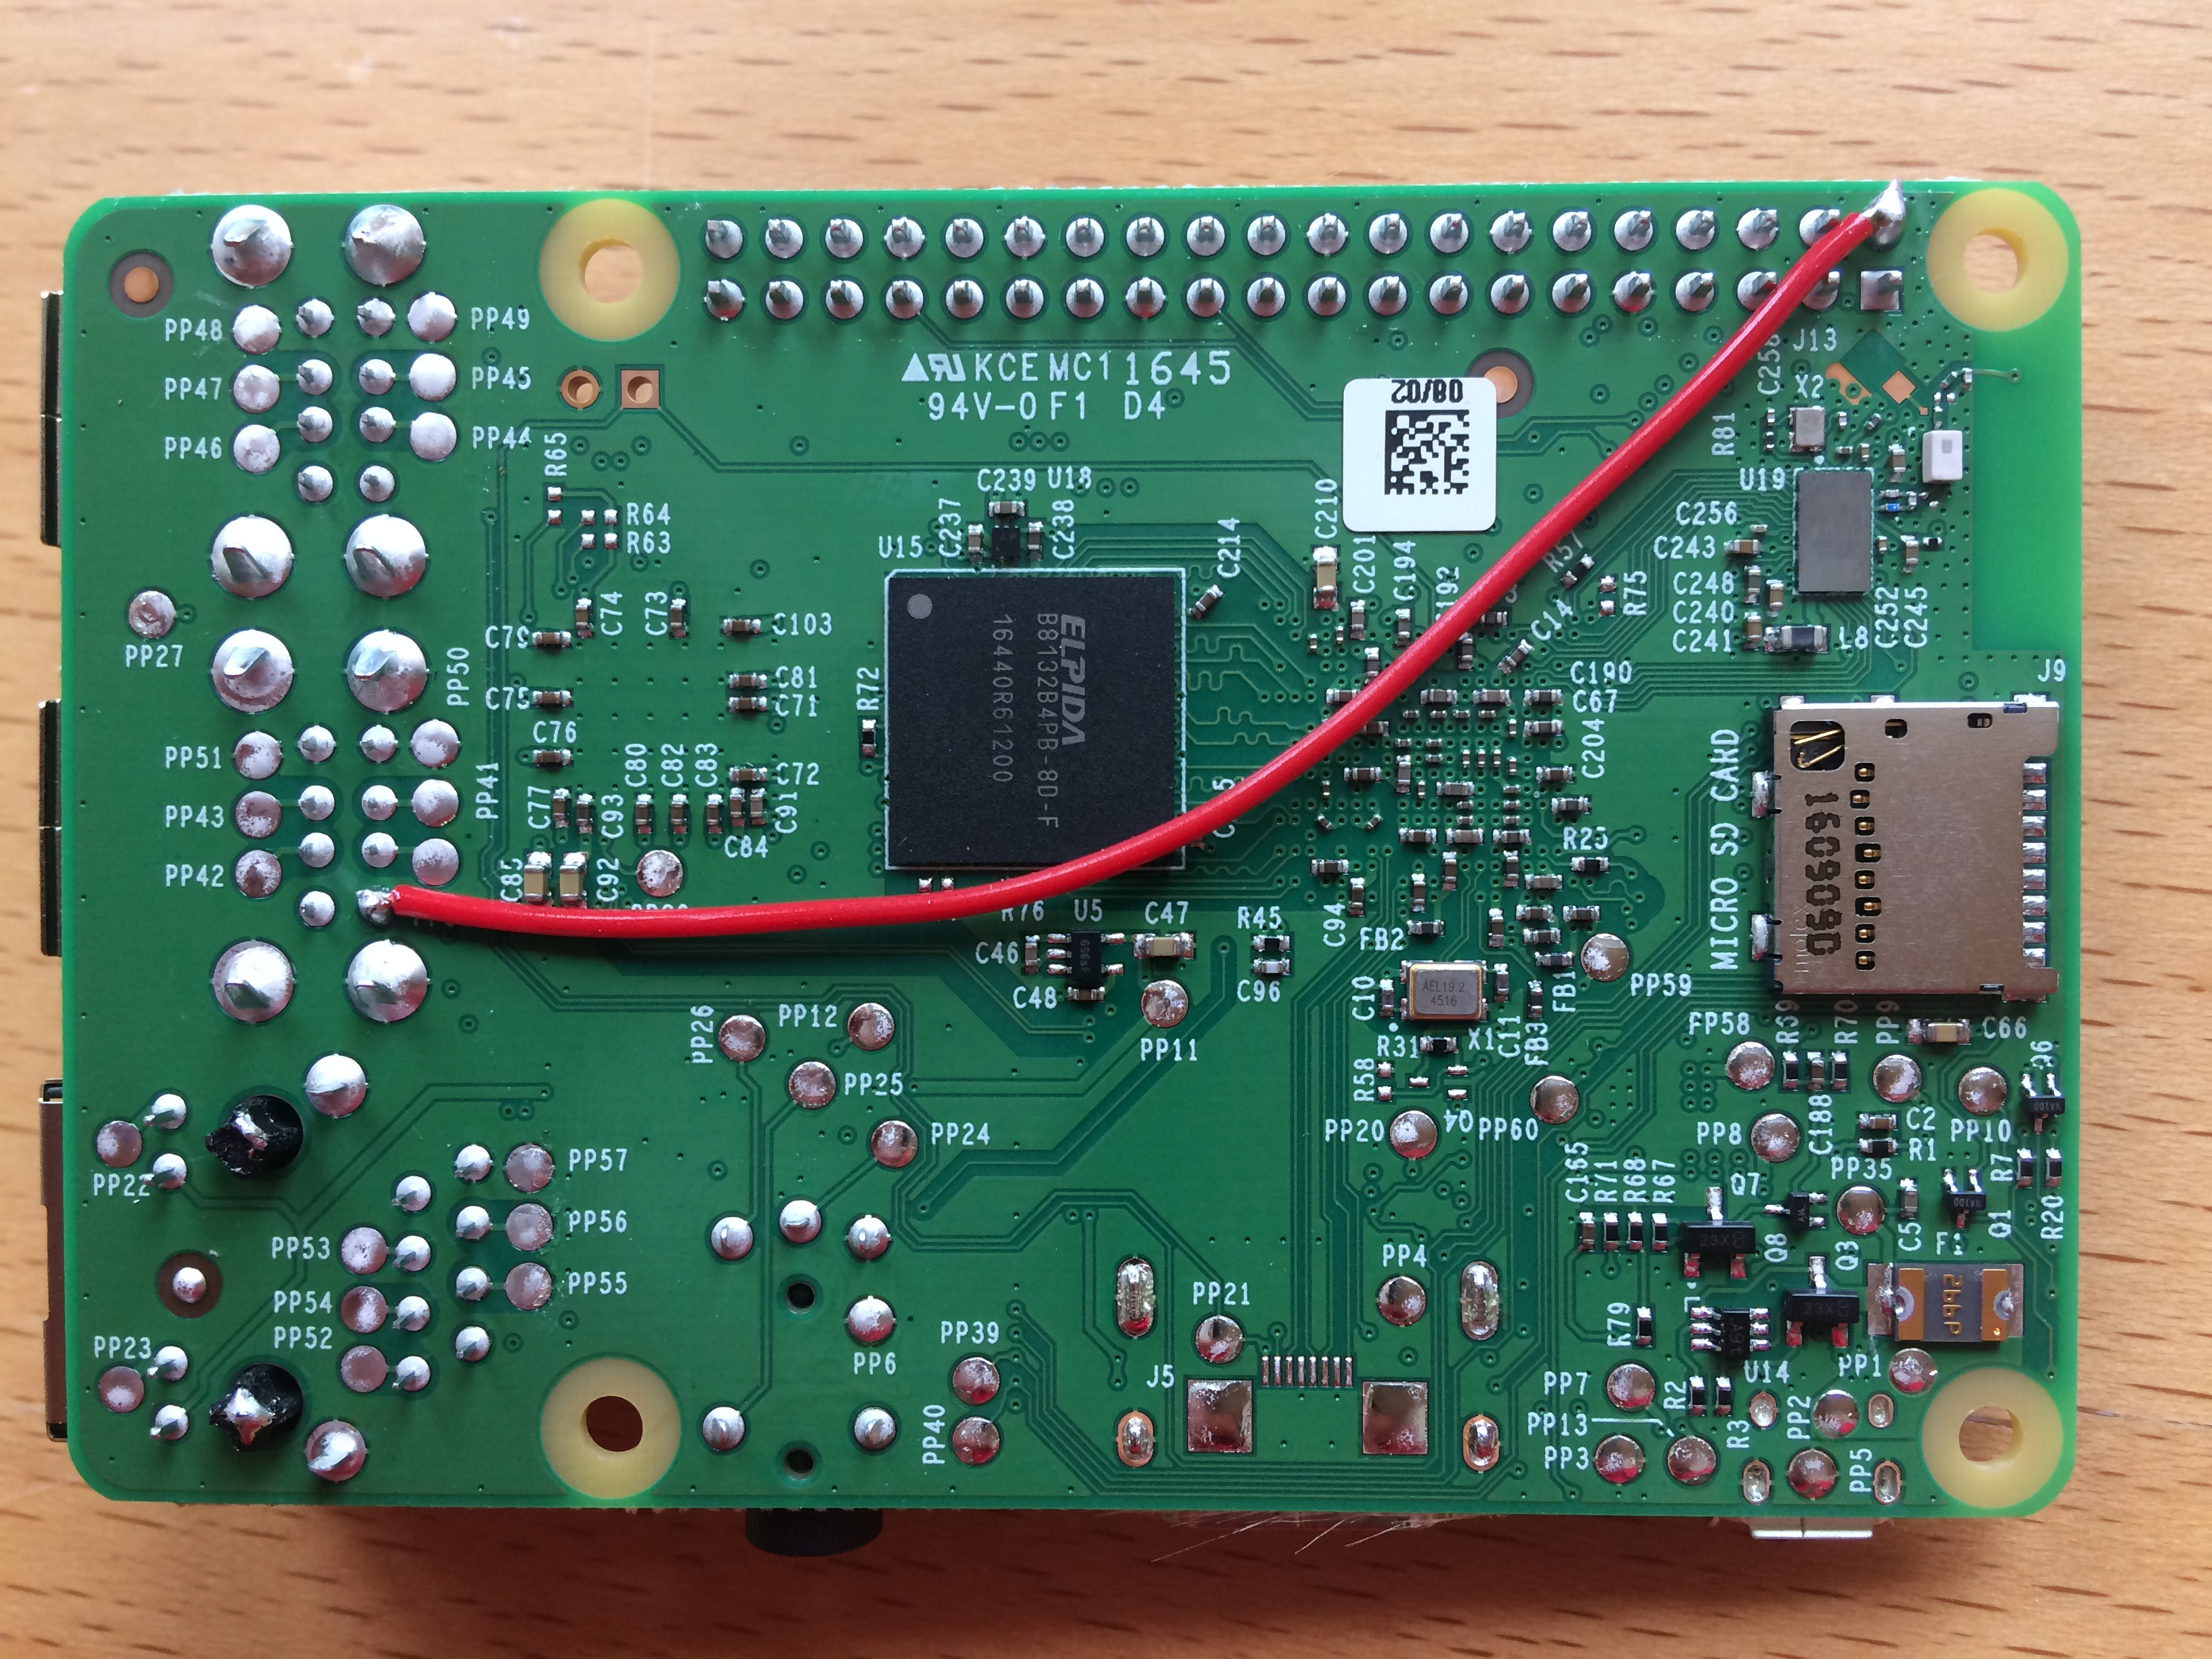
\includegraphics[width=\textwidth]{./photos/Pi2.JPG}
\end{minipage}
\begin{minipage}{0.66\textwidth} %% Text Modified raspberry pi
  These picture show a top and bottom view of a modified Raspberry
  Pi. The modification is a wire soldered from the 5V pin on the USB
  port to the Pi 5V net. The Pi's own voltage regulator transforms
  this to the 3.3V needed.
\end{minipage}

\todo{Maybe a picture of the little radio tranceiver (The mote?) ?}

\todo{A picture showing what features these provides and how they
  connect (something like in the paper)}


\section{Configuring a Linux Machine}

This section describes how to set up a linux system (an Ubuntu system
is assumed) with the tools needed to run RControlStation and to
develop towards the RISE SDVP. Start out by installing some basic
dependencies:

\begin{Verbatim}
\sudo apt-get install git build-essential libudev-dev
\end{Verbatim}

The IDEs (development environments) preferred by some of the authors of
this documentation is Qt-Creator and Eclipse. To download Eclipse
click
\href{http://ftp-stud.fht-esslingen.de/pub/Mirrors/eclipse/oomph/epp/photon/R/eclipse-inst-linux64.tar.gz}{here}
\footnote{\texttt{\tiny{wget
      http://ftp-stud.fht-esslingen.de/pub/Mirrors/eclipse/oomph/epp/photon/R/eclipse-inst-linux64.tar.gz}}}.
Qt can be downloaded from \url{https://www.qt.io/download} or click
\href{http://download.qt.io/official_releases/online_installers/qt-unified-linux-x64-online.run}{here}
to directly download the open source version. Now, install Qt and
Eclipse, both have install wizards to help with this procedure. 

Arm development tools are needed if you want to compile new versions
of the various firmwares for the microcontrollers on the
SDVP. Download arm development tools from \url{developer.arm.com} or
click this
\href{https://developer.arm.com/-/media/Files/downloads/gnu-rm/7-2018q2/gcc-arm-none-eabi-7-2018-q2-update-linux.tar.bz2?revision=bc2c96c0-14b5-4bb4-9f18-bceb4050fee7?product=GNU%20Arm%20Embedded%20Toolchain,64-bit,,Linux,7-2018-q2-update}{link}. 
  To install the ARM tools simply extract the files from the archive
  and place them in a suitable location, for example \texttt{\$HOME/opt/gcc-arm-none-eabi/}.
\begin{Verbatim}
  tar xvf gcc-arm-none-eabi-7-2018-q2-update-linux.tar.bz2
  mv gcc-arm-none-eabi-7-2018-q2-update-linux $HOME/opt/gcc-arm-none-eabi
\end{Verbatim} 
Then configure your \texttt{\$PATH} path variable to include \texttt{\$HOME/opt/gcc-arm-none-eabi/bin}

OpenOCD is used To flash the ARM Cortex M4 microcontrollers used throughout the SDVP.
To install OpenOCD execute the following command: 
\begin{Verbatim}
sudo apt-get install openocd
\end{Verbatim} 

Add yourself to the {\em dialout} group to be able to use, for example
{\texttt ttyACM0} without having to be root user (sudo). This is useful when connecting to
the various sdvp boards over a serial link (USB). 
\begin{Verbatim}
sudo usermod -a -G dialout <USER_NAME> 
\end{Verbatim}
After adding yourself to the dialout group, you need to log out and in again
for the change to take effect. 

It can also be good to uninstall modemmanager, if installed, as it sometimes leads to confusing the
system for a while when connecting over serial port.
\begin{Verbatim}
sudo apt-get remove modemmanager
\end{Verbatim}

Your Linux system is now set up for SDVP development (and use). The
next step is to clone the rise\_sdvp repository from github. Executing the
following command will create a new directory called rise\_sdvp, so make sure
are already in a suitable directory:
\begin{Verbatim}
cd <SUITABLE_DIR>   
git clone git@github.com:vedderb/rise_sdvp
\end{Verbatim}
The directory \texttt{<SUITABLE\_DIR>/rise\_sdvp} will in the rest of the document
be referred to as the \texttt{<SDVP\_DIR>}.


\section{Buidling RControlStation}

To build and run RControlStation, start Qt-Creator and on the welcome
screen click {\em Open Project}. Navigate in the directory hierarchy
to where you cloned the rise\_sdvp repository and go to
\texttt{<SDVP\_DIR>/Linux/RControlStation}. Select the file
\texttt{RControlStation.pro} and click open. Qt-Creator will now open
the project and switch to a new view that allows you to edit files.
On the left side of the window you can browse the RControlStation
project.  To build, locate the {\em Build} menu and select {\em Build
  Project ``RControlStation''}.  At the bottom of the Qt-Creator
window there is a collection of tabs, one of them reads {\em 4 Compile
  Output}. You can keep an eye on this tab for any error outputs
during compilation. 

When compilation concludes successfully, click the little green
``play'' button located along the left edge of Qt-Creator. This should
bring up RControlStation.

\section{RControlStation GUI}

When RControlStation starts up you should be presented with a view very similar to
this:
\noindent 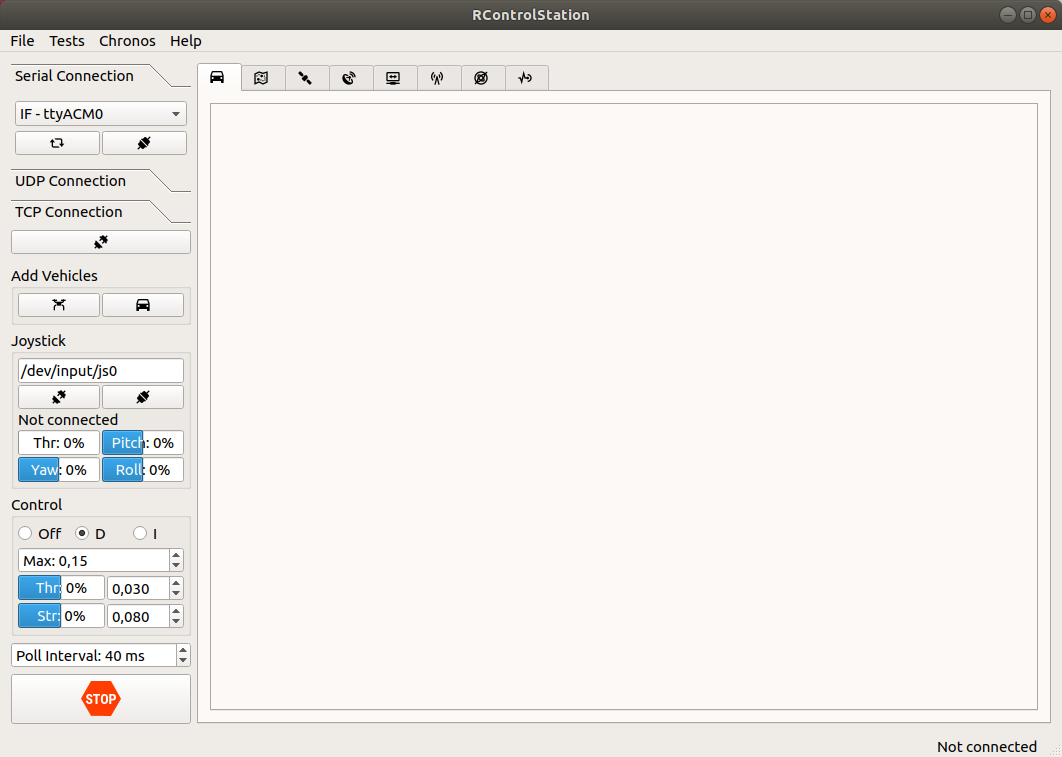
\includegraphics[width=\textwidth]{./screens/RControlStation1.png}
In this section we will go through and briefly explain the meaning and functionality
behind most of the elements of this GUI.

%\subsection{Menu Bar}

%\noindent 
\includegraphics[width=0.3\textwidth]{./screens/menubar1.png}
%It just feels silly to try and explain this. 


%% \noindent {\bf File:} 
%% \begin{itemize}
%% \item Save Routes
%% \item Save Routes with IDs
%% \item Load Routes
%% \item Exit
%% \end{itemize}

%% \noindent {\bf Tests:}
%% \begin{itemize}
%% \item Intersection
%% \item GPS Simulator
%% \end{itemize} 

%% \noindent {\bf Chronos:}
%% \begin{itemize}
%% \item Save selected route as drive file
%% \item Load drive file
%% \end{itemize}

%% \noindent {\bf Help:}
%% \begin{itemize}
%% \item About
%% \item About Libraries Used
%% \item About Qt
%% \end{itemize}



\subsection{Connectivity Controls}


\noindent \begin{minipage}{0.2\textwidth}
  \noindent 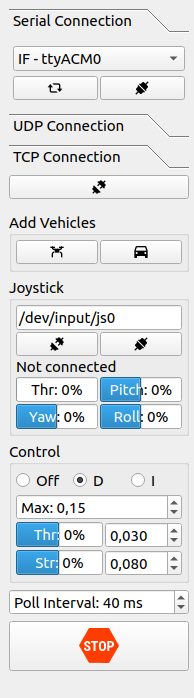
\includegraphics[width=\textwidth]{./screens/Left_controls1.png}
\end{minipage}
\begin{minipage}{0.7\textwidth}
  To the left side of RControlStation are fields for selection method of connecting to the
  SDVP, adding vehicles and control related configuration and indicators.  
  \begin{itemize}
  \item {\bf Connection:} Serial, UDP or TCP connection can be
    selected. Serial is used when connecting to the RTK controller
    using the radio mote or directly via USB cable. UDP and TCP
    connects to the SDVP via Raspberry Pi using either WIFI or 4G.
    Below the connection tabs is a button for disconnecting whatever
    connection has been set up. 
  \item {\bf Add Vehicles:} Add a car or quadcopter. Adding for
    example a car, changes the view on the right side to display a car
    and its set of car specific controls. The car specific controls are
    shown in Section~\ref{sec:cars} and quadcopter controls in Section\ref{sec:quads}.
  \item {\bf Joystick:} 
  \item {\bf Control:} Is related to the keyboard control
    functionality. It can be turned off, put in ``D'' mode or ``I''
    mode. ``D'' refers to duty mode and ``I'' representing current
    mode.  A ``gain'' value can be set for thrust and steering that
    influences how strongly these respond to keyboard interaction.
  \item {\bf Poll Interval:}
  \item {\bf Stop:} Stops a moving car that is running under auto pilot.
  \end{itemize} 
\end{minipage}


\subsection{Cars}
\label{sec:cars}

%% ------------------------------------------------------------

  After adding a car, ``Car 0'' will appear in the {\em Cars} tab with
  a set controls similar to this image.  To the right of the displayed
  3D image of a car is a set of controls, toggles and buttons, the
  ``Car ID'' field should be set so that it corresponds to the setting
  of the dip switches on the RTK controller. A way to test if the
  connection to the car is working, is to check the {\bf Poll data}
  box and checking if the rendered image of the car seems to respond
  to moving of the actual car.
  
\noindent \begin{minipage}{0.5\textwidth}
    \noindent 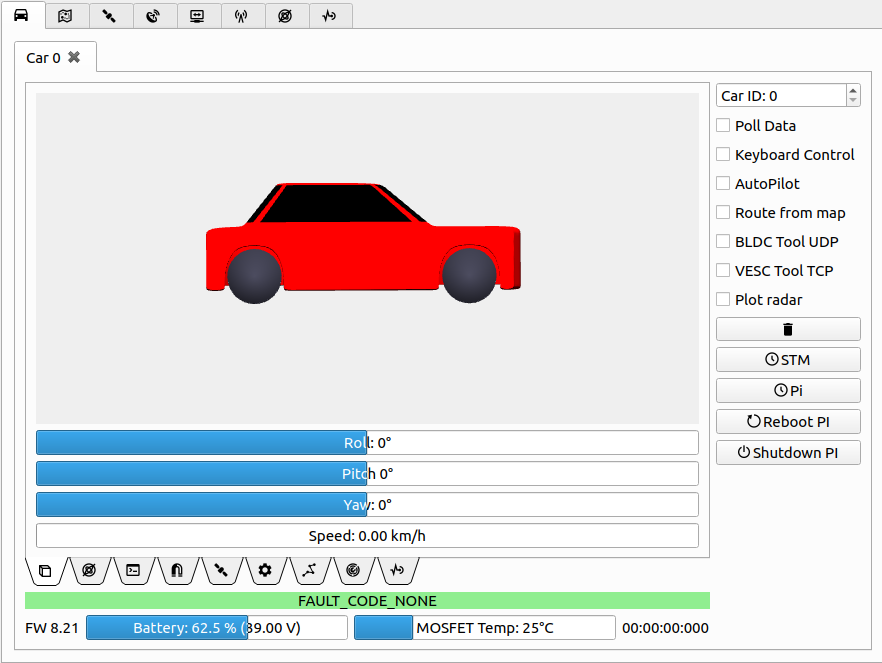
\includegraphics[width=\textwidth]{./screens/Car_orientation.png}
\end{minipage}
\begin{minipage}{0.5\textwidth} %% Text Car orientatio

  Toggling {\bf Keyboard Control} allows control of the car via the
  keyboard arrow keys and {\bf AutoPilot} starts trajectory following
  mode.

  The {\bf Route from map} toggle, turns on or off direct upload of
  trajectory points to the car as they are added to the map.

  The next two toggles, {\bf BLDC Tool UDP} and {\bf VESC Tool TCP}
  start servers for interfacing with external tools. 

  {\bf Plot radar} turns plotting of radar samples on. Note that a
  radar is not part of the standard setup of an RISE SDVP car.
\end{minipage}

There is a set of indicator bars under the 3D model of the car showing
pitch, roll and yaw degrees and a speed display. Then there is a set
of tabs for further configurations or interfacing, these tabs are all
explained below.

%% ------------------------------------------------------------

%% ------------------------------------------------------------
\noindent\begin{minipage}{0.5\textwidth} %% Text Car IMU

The IMU tab displays realtime sensor data from the Inertial
Measurements Unit. The top graph shows accelerometer readings,
measured in G:s, in the middle gyroscope readings in degrees per
second are displayed and at the bottom the magnetometer data in micro
Teslas.

\end{minipage}
\begin{minipage}{0.5\textwidth}
      \noindent 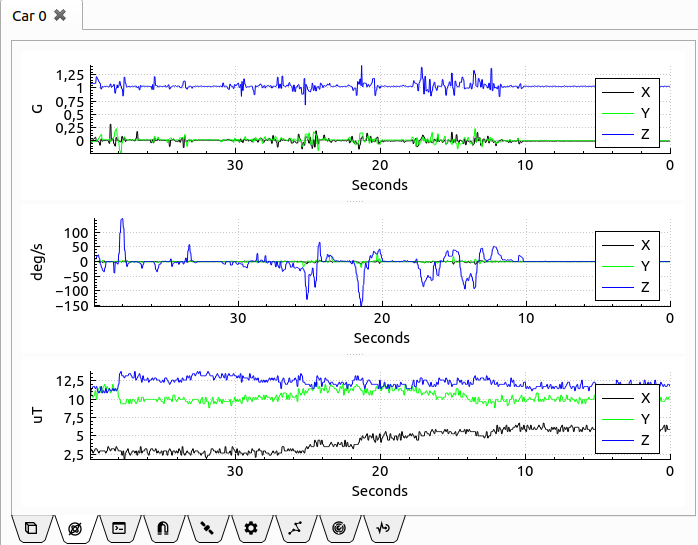
\includegraphics[width=\textwidth]{./screens/Car_IMU_realtime.png}
\end{minipage}
%% ------------------------------------------------------------


%% ------------------------------------------------------------
\noindent\begin{minipage}{0.5\textwidth}
  \noindent 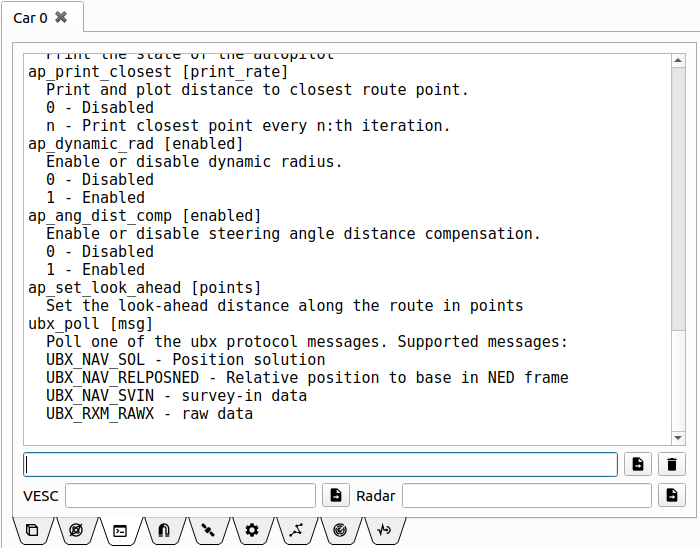
\includegraphics[width=\textwidth]{./screens/Car_terminal.png}
\end{minipage}
\begin{minipage}{0.5\textwidth} %% Text Car terminal interface
  This tab provides a terminal interface to the car. The ``help'' commands provides a list
  of valid commands. Section~\ref{sec:terminalcommands} shows a list of commands that
  are valid at 2018-09-03. 
\end{minipage}


%% ------------------------------------------------------------


%% ------------------------------------------------------------
\noindent\begin{minipage}{0.5\textwidth} %% Text Car calibration On
On this tab there are controls for steering servo and magnetometer
calibration.  To callibrate the magnetometer, turn on {\bf poll data}
and check the store samples box. There are buttons for calculating
compensation, loading and storing of samples and to view C code
representing the calibrations settings.

\todo{Needs improvement}

\end{minipage}
\begin{minipage}{0.5\textwidth}
  \noindent 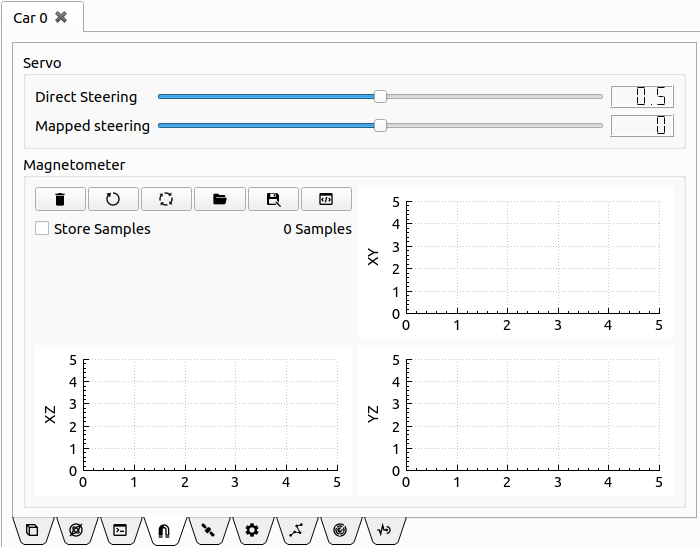
\includegraphics[width=\textwidth]{./screens/Car_calibration.png}
\end{minipage}
%% ------------------------------------------------------------

%% ------------------------------------------------------------
\noindent\begin{minipage}{0.5\textwidth}
  \noindent 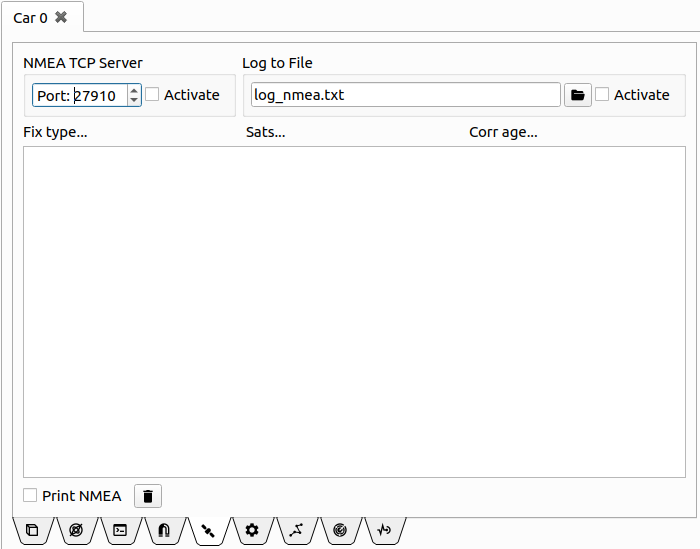
\includegraphics[width=\textwidth]{./screens/Car_GPS.png}
\end{minipage}
\begin{minipage}{0.5\textwidth} %% Text Car GPS
  \todo{text}
\end{minipage}
%% ------------------------------------------------------------

%% ------------------------------------------------------------
\noindent\begin{minipage}{0.5\textwidth} %% Text Car Configuration

The {\em Car Settings} tab contains configurations that can be loaded
and stored to the car. Loading and storing is done using the up and
down arrow buttons located at the bottom right. The preferred way of
changing these is to first load the current settings from the car with
the up button, then perform changes followed by writing the
configuration back to the car. Changing the information in the top
half of this tab requires knowledge of the dynamics of the car.

The bottom half of this tab contains a number of sub-tabs that are
explained below.
\end{minipage}
\begin{minipage}{0.5\textwidth}
  \noindent 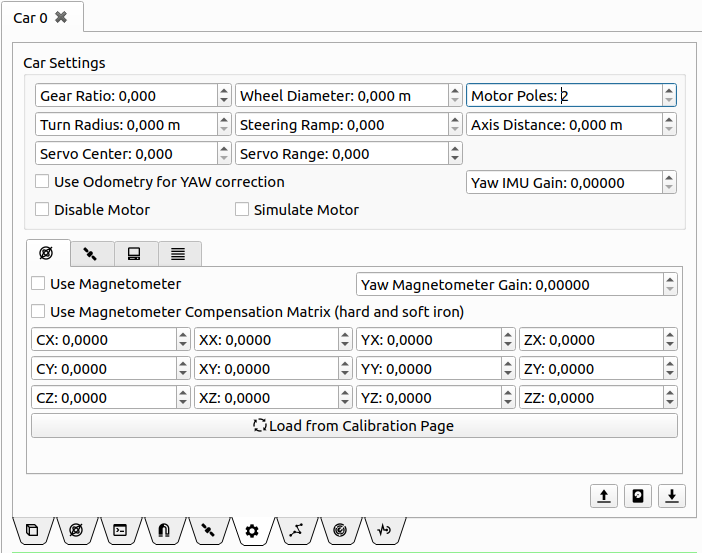
\includegraphics[width=\textwidth]{./screens/Car_configuration.png}
\end{minipage}
%% ------------------------------------------------------------
\noindent\begin{minipage}{0.4\textwidth}
\noindent 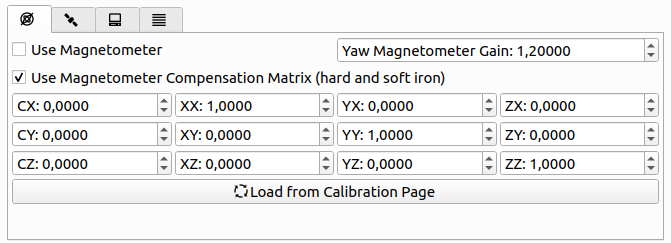
\includegraphics[width=\textwidth]{./screens/car_settings_mag.png}
\noindent 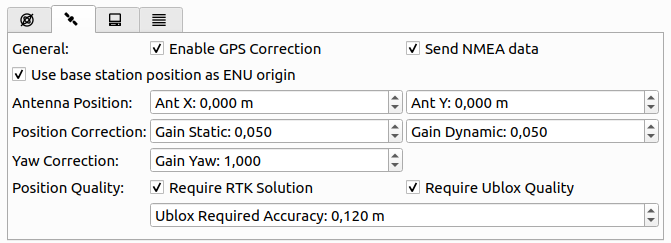
\includegraphics[width=\textwidth]{./screens/car_settings_gps.png}
\noindent 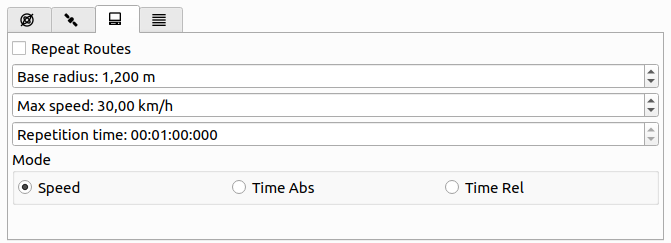
\includegraphics[width=\textwidth]{./screens/car_settings_auto.png}
\noindent 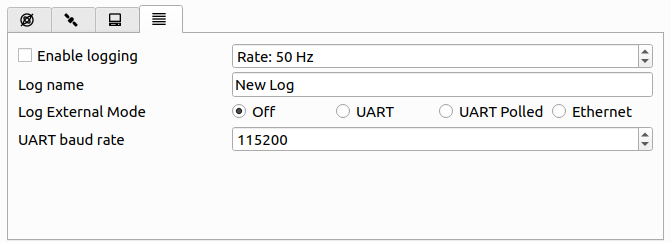
\includegraphics[width=\textwidth]{./screens/car_settings_log.png}
\end{minipage}
\begin{minipage}{0.7\textwidth} %% Text Car Experiment
\noindent {\bf Magnetometer:} Turn usage of magnetometer data on or
offf and configure compensation matrix.

\noindent {\bf GPS:} \todo{ Write }

\noindent {\bf AutoPilot:} Configure the behaviour of the auto
pilot. If the car should repeat the route after completion check the
{\em Repeat Route} box. The {\em Base Radius} setting is related to
the variant of the PurePersuit algorithm used for trajectory following
where the car heads towards the closest point intersecting the
trajectory on a circle surrounding the car. There are also three
different modes for trajectory following: in {\em Speed} mode the car
uses speed information stored in the trajectory, then there is
absolute time and relative time where timestamps on the trajectory
either are treated as an absolute time when car should be at point or
time relative to previous point.

\noindent {\bf Logging:} Enable, disable and set frequence of logging. There is
also an {\em External} mode where the log data is sent over for example UART.
\todo{Fill in more details of how this works}.
\end{minipage}
%% ------------------------------------------------------------
\noindent\begin{minipage}{0.6\textwidth}
  \noindent 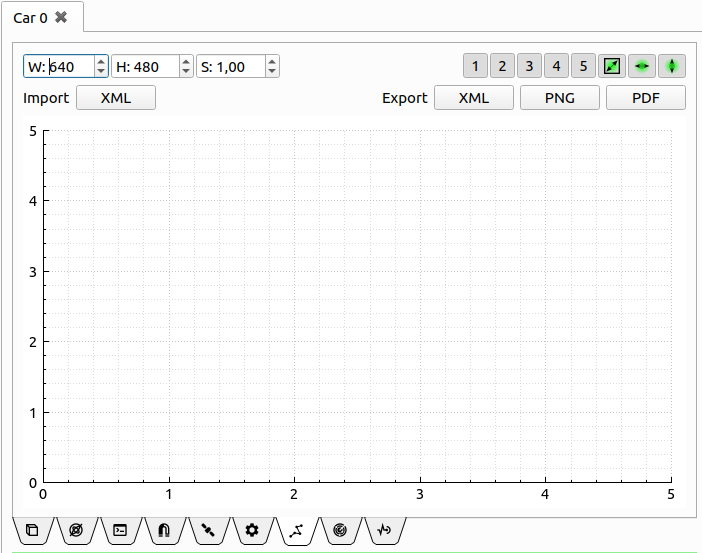
\includegraphics[width=\textwidth]{./screens/Car_experiment_plot.png}
\end{minipage}
\begin{minipage}{0.5\textwidth} %% Text Car Experiment
  \todo{text}
\end{minipage}
%% ------------------------------------------------------------

%% ------------------------------------------------------------
\noindent\begin{minipage}{0.5\textwidth} %% Text Car Radar
  \todo{text}
\end{minipage}
\begin{minipage}{0.5\textwidth}
  \noindent 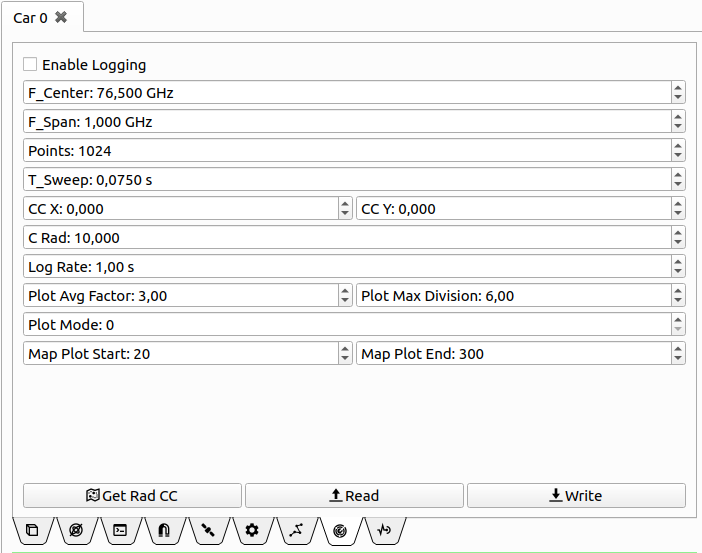
\includegraphics[width=\textwidth]{./screens/Car_radar.png}    
\end{minipage}
%% ------------------------------------------------------------


%% ------------------------------------------------------------
\noindent\begin{minipage}{0.5\textwidth}
  \noindent 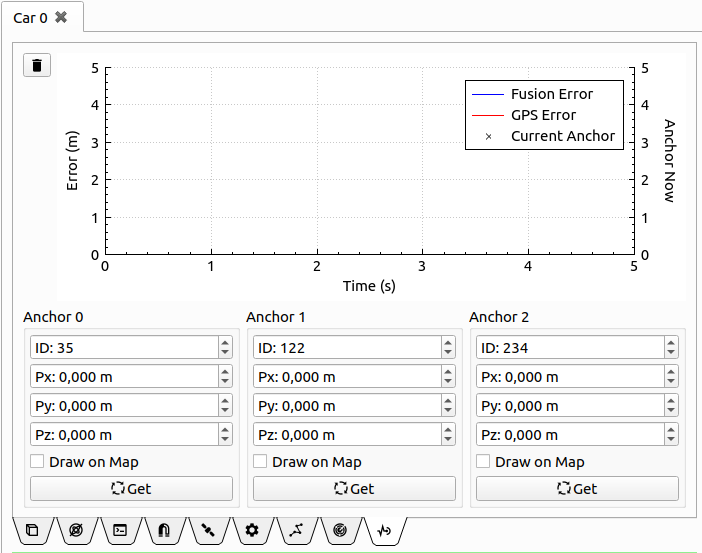
\includegraphics[width=\textwidth]{./screens/Car_UWB.png}
\end{minipage}
\begin{minipage}{0.5\textwidth} %% Text Car UWB
  This tab allows the configuration of three UWB anchors and also displays a plot
  of relative error at time.
  \begin{itemize}
  \item {\bf ID:} Corresponds to an ID coded into the firmware or the UWB anchor.
  \item {\bf Px,Py, Pz:} Position of the anchor. The {\em Get} button
    reads the current position of the car into these fields. 
  \end{itemize} 
\end{minipage}
%% ------------------------------------------------------------


\subsection{Quadcopters}
\label{sec:quads}

%% ------------------------------------------------------------
\noindent\begin{minipage}{0.5\textwidth}
  \todo{text}
\end{minipage}
\begin{minipage}{0.5\textwidth}
  \noindent 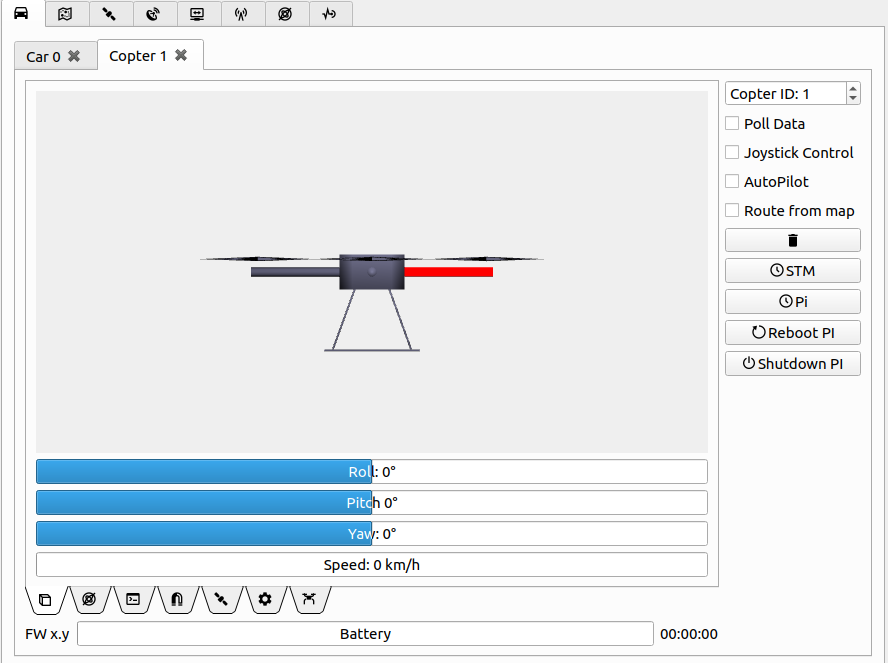
\includegraphics[width=\textwidth]{./screens/quad_orientation.png}
\end{minipage}
%% ------------------------------------------------------------


%% ------------------------------------------------------------
\noindent\begin{minipage}{0.5\textwidth}
  \noindent 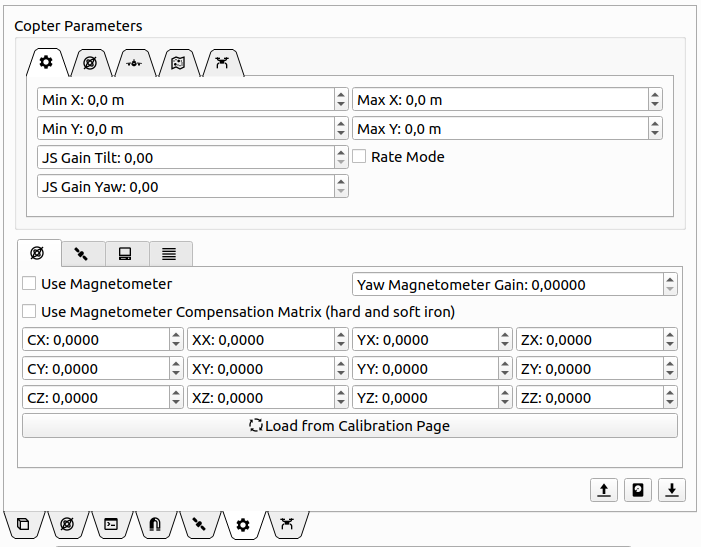
\includegraphics[width=\textwidth]{./screens/Quad_parameters.png}
\end{minipage}
\begin{minipage}{0.5\textwidth}
  \todo{text}
\end{minipage}
%% ------------------------------------------------------------

%% ------------------------------------------------------------
\noindent\begin{minipage}{0.5\textwidth}
  \todo{text}
\end{minipage}
\begin{minipage}{0.5\textwidth}
  \noindent 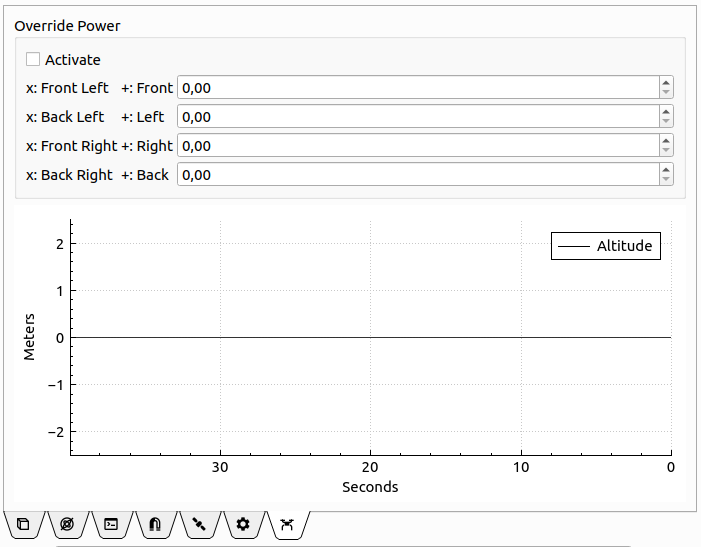
\includegraphics[width=\textwidth]{./screens/Quad_tests.png}
\end{minipage}
%% ------------------------------------------------------------


\subsection{Map}

This tab shows a map based on OpenStreetMap overlaid with a grid
showing distances from an origo. The origo is set to the ENU (East
North Up) reference point used in positioning calculations. This ENU
point can be configured to be postion of the GNSS-RTK base station.

To zoom in or out on the map use the scrollwheel on the mouse or two
fingers on the touchpad. Panning is done by clicking and dragging
with the mouse. The following keyboard shortcuts are also useful for
interaction the map view:

\noindent\begin{minipage}{0.5\textwidth}
  \noindent 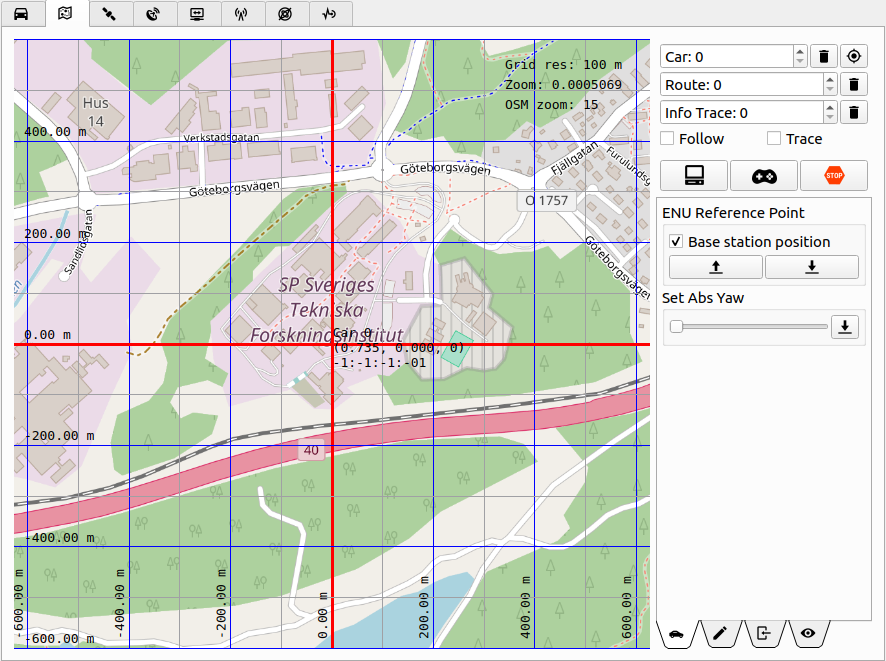
\includegraphics[width=\textwidth]{./screens/map_car_control.png}
\end{minipage}
\noindent\begin{minipage}{0.5\textwidth}
\begin{itemize} 
  \item {\bf CTRL + Right click:} Update route point or anchor settings
  \item {\bf Shift + Left click:} Add route point or anchor
  \item {\bf Shift + Left drag:} Move route point or anchor
  \item {\bf Shift + right click:} Delete route point or anchor
  \item {\bf CTRL + SHIFT + Left click:} Zero map ENU coordinates
\end{itemize}
\end{minipage}

\noindent\begin{minipage}{0.25\textwidth}
\noindent 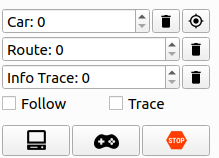
\includegraphics[width=\textwidth]{./screens/map_top_right.png}
\end{minipage}
\noindent\begin{minipage}{0.75\textwidth} These controls to the right
of the map allows selections of car, route and trace based on
ID. Checking the {\em Follow} box results in the map following the
selected cars movements automatically. The buttons are for turning
auto pilot, manual control and stopping a car running on auto pilot.
\end{minipage} 

Below to the right, there is a set of tabs with controls and
configurations for use together with the map. The first of these tabs
is called {\em Car Control}


\noindent\begin{minipage}{0.25\textwidth}
\noindent 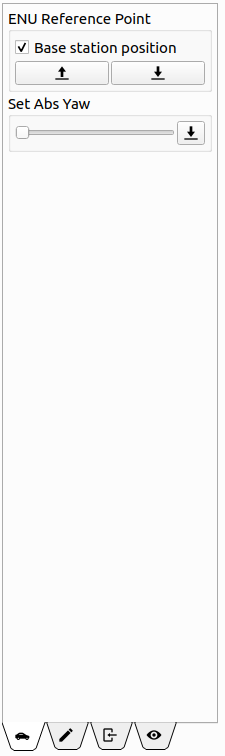
\includegraphics[width=\textwidth,height=12cm]{./screens/map_car_control_panel2.png}
\end{minipage}
\noindent\begin{minipage}{0.75\textwidth} This tab lets you load base
station position from the car or store an updated one (from the map
view) to the car. \todo{What is Abs yaw?} 
\end{minipage}


%\begin{minipage}{0.25\textwidth}
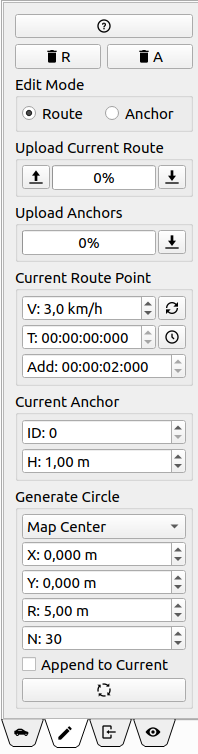
\includegraphics[width=0.25\textwidth,height=12cm]{./screens/map_edit_panel.png}
%\end{minipage}
%\begin{minipage}{0.25\textwidth}
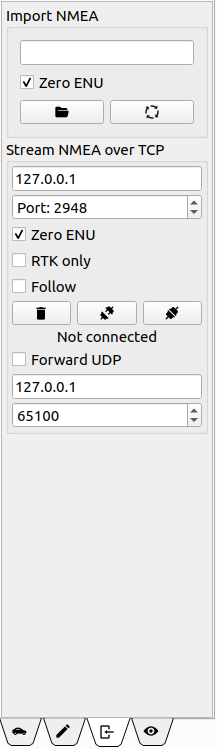
\includegraphics[width=0.25\textwidth,height=12cm]{./screens/map_import_panel.png}
%\end{minipage}
%\begin{minipage}{0.25\textwidth}
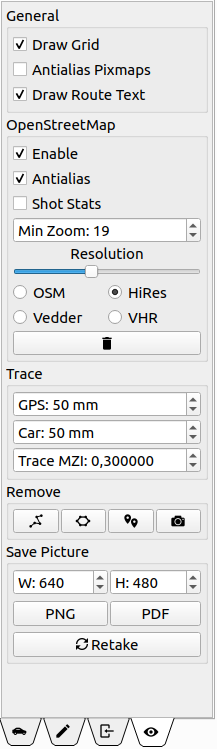
\includegraphics[width=0.25\textwidth,height=12cm]{./screens/map_view_panel.png}
%\end{minipage}

\subsection{RTCM Client}

\noindent 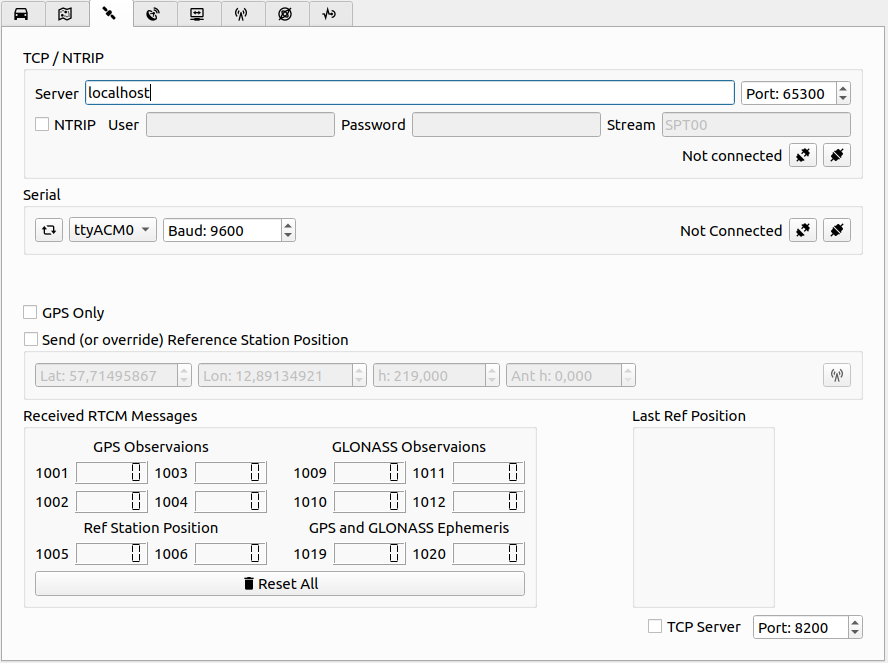
\includegraphics[width=\textwidth]{./screens/RTCM_client.png}

\todo{Write}

\subsection{Base Station}

\noindent 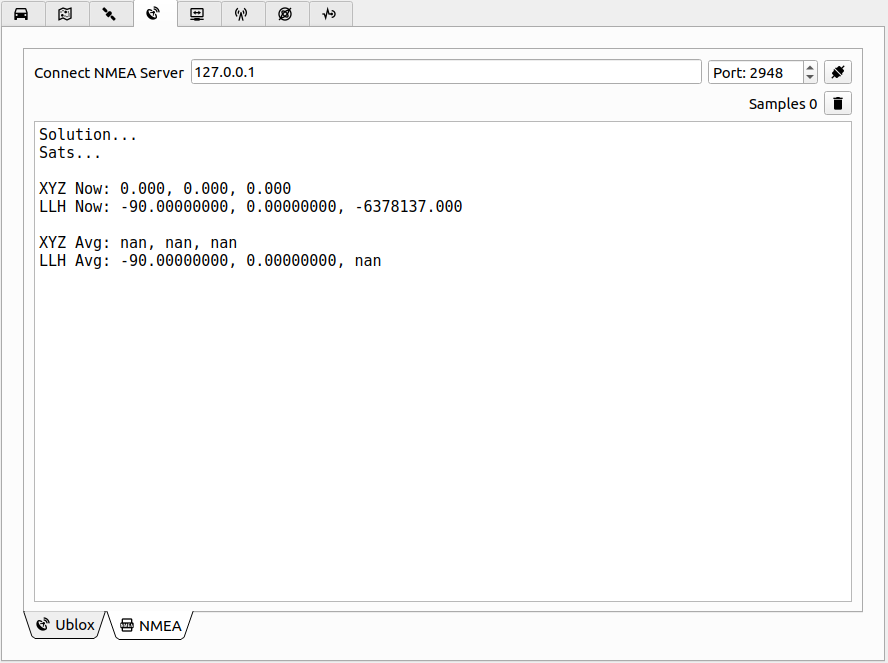
\includegraphics[width=\textwidth]{./screens/base_station_NMEA.png}

\noindent 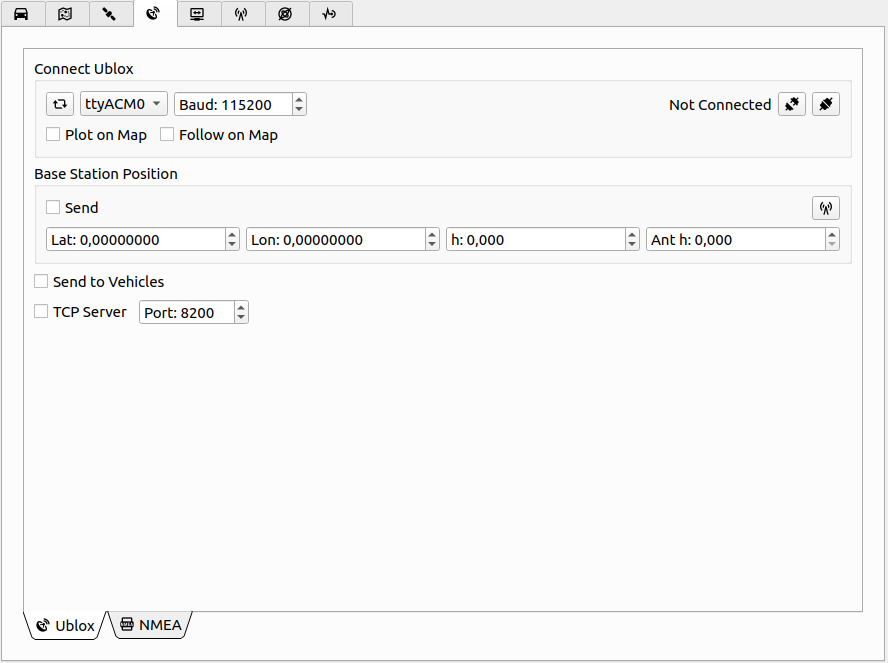
\includegraphics[width=\textwidth]{./screens/base_station_UBLOX.png}

\todo{Write}

\subsection{Network Interface}

\noindent 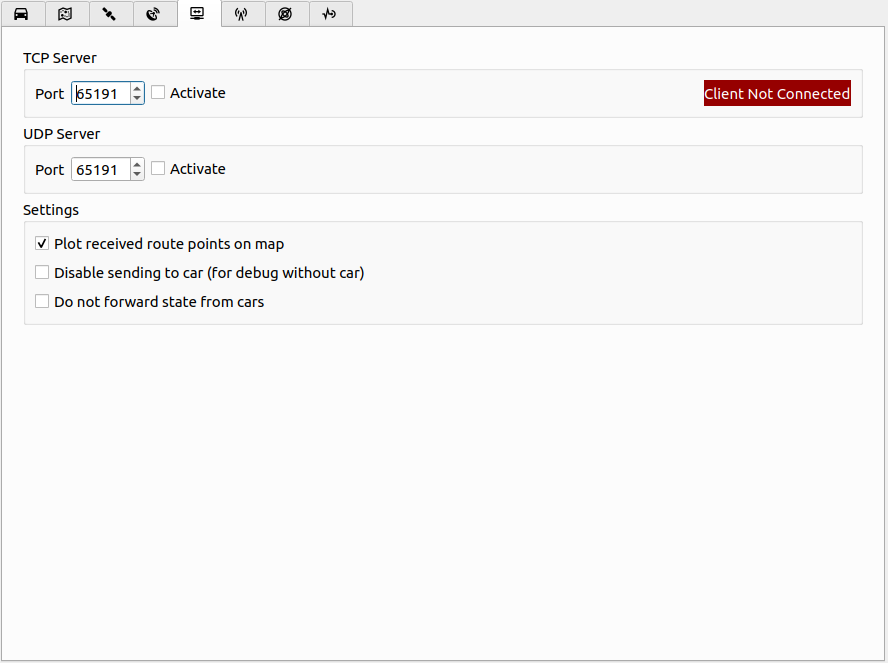
\includegraphics[width=\textwidth]{./screens/network_interface.png}

\todo{Write}

\subsection{Mote}

\noindent 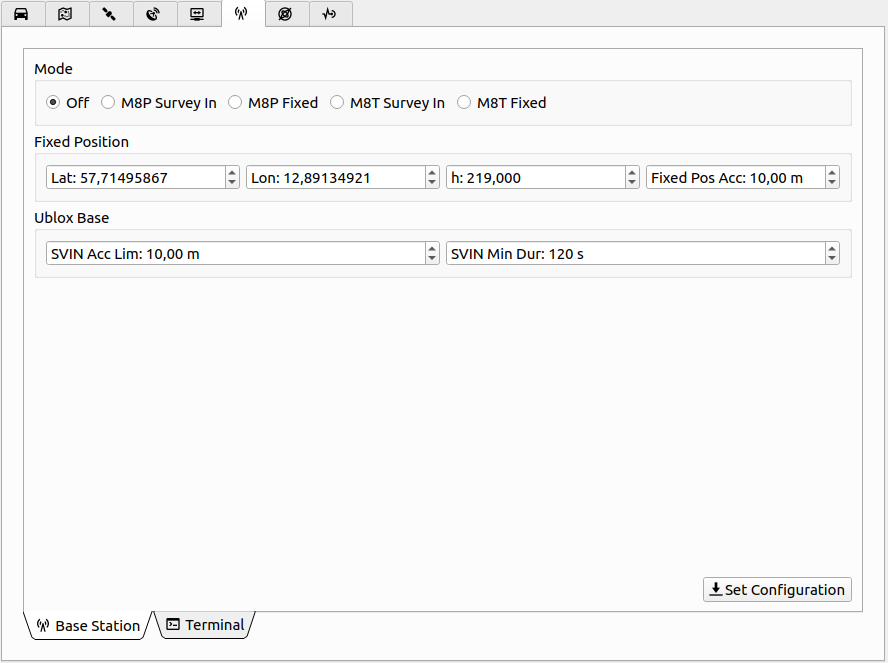
\includegraphics[width=\textwidth]{./screens/mote.png}

\todo{Write}

\subsection{NCom CLient}

\noindent 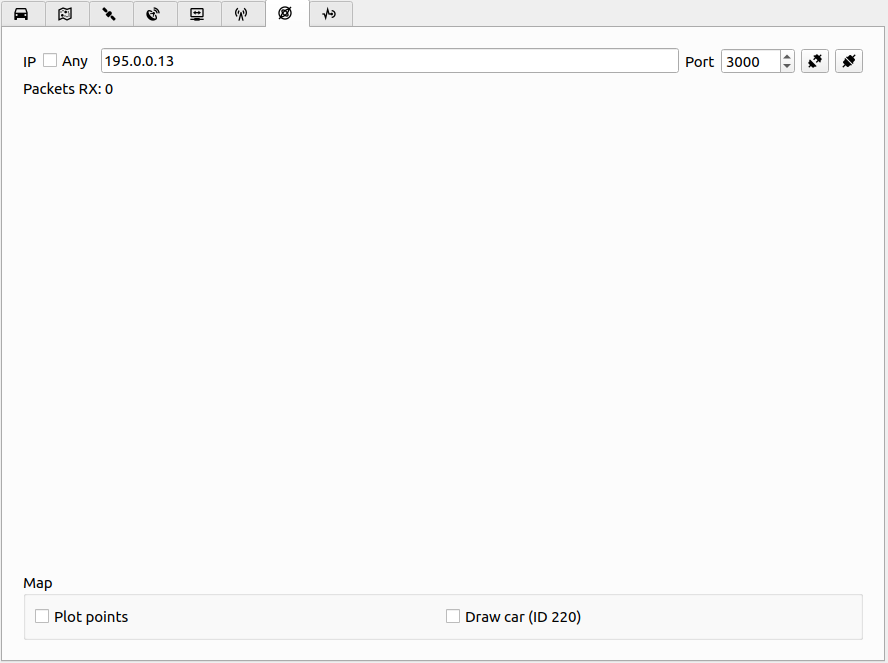
\includegraphics[width=\textwidth]{./screens/ncom_client.png}

\todo{Write}

\subsection{Logging and Analysis}

\noindent 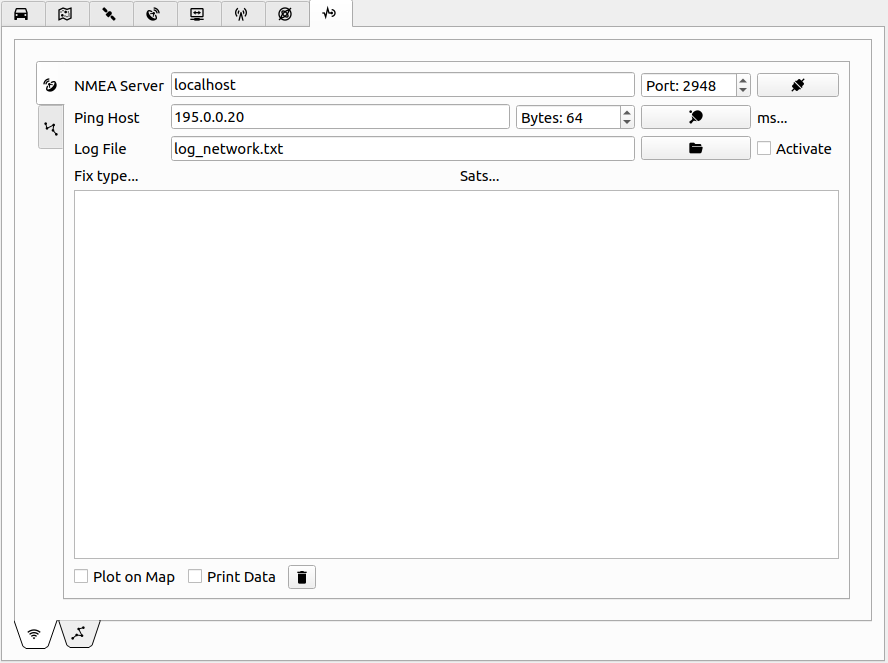
\includegraphics[width=\textwidth]{./screens/Log1.png}

\noindent 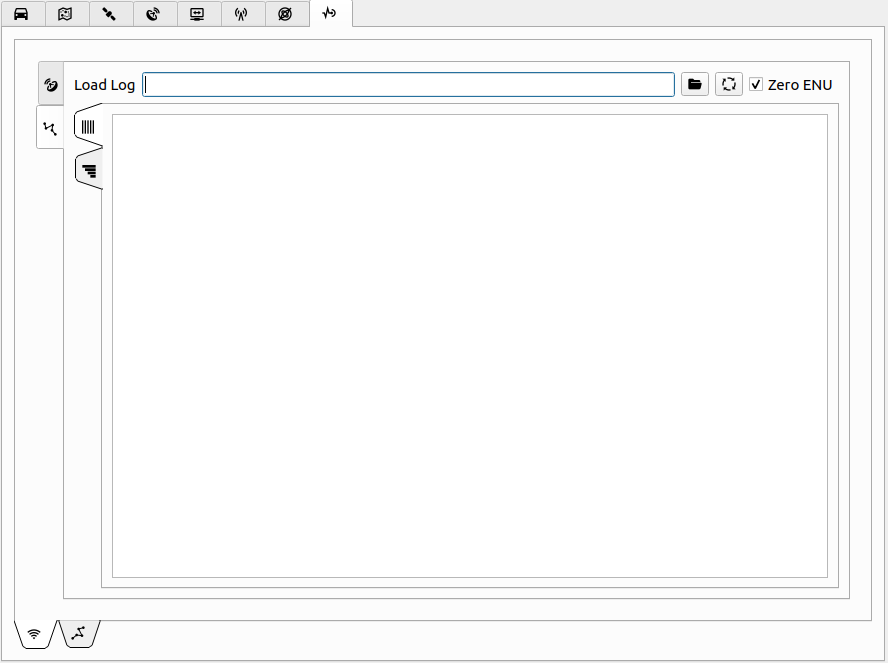
\includegraphics[width=\textwidth]{./screens/Log2.png}

\noindent 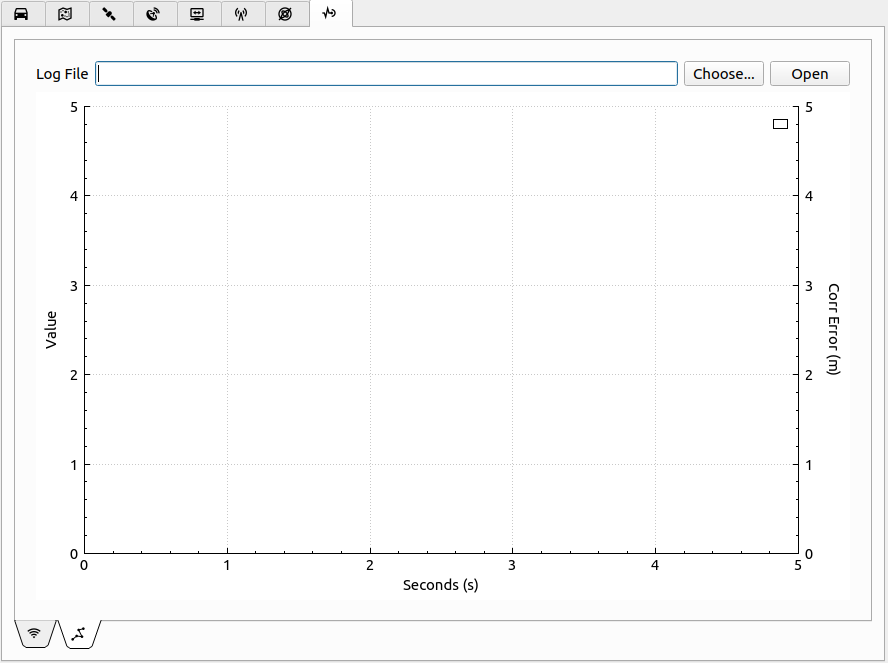
\includegraphics[width=\textwidth]{./screens/Log3.png}

\todo{Write}

\section{Example Setup: HIL Simulation Rig}

\todo{Write}

\section{Example Setup: Fully Operational System}

\todo{Write}

\section{Take a Test Drive}

\todo{Something like this:}
\begin{itemize}
\item What to look at (GPS fix?)
\item Set up a trajectory
\item run autopilot
\item be ready to abort
\item .... what else ? 
\end{itemize} 





\section{RControlStationComm Library}

\todo{Write}
\subsection{C++ library}

\begin{Verbatim}
class RCONTROLSTATIONCOMMSHARED_EXPORT RControlStationComm
{

public:
    RControlStationComm();
    ~RControlStationComm();
    bool connectTcp(QString host, int port);
    void disconnectTcp();
    void setDebugLevel(int level);
    bool hasError();
    char *lastError();
    bool getState(int car, CAR_STATE *state, int timeoutMs = 1000);
    bool getEnuRef(int car, bool fromMap, double *llh, int timeoutMs = 1000);
    bool setEnuRef(int car, double *llh, int timeoutMs = 1000);
    bool addRoutePoints(int car, ROUTE_POINT *route, int len,
                        bool replace = false, bool mapOnly = false,
                        int mapRoute = -1, int timeoutMs = 1000);
    bool clearRoute(int car, int mapRoute = -1, int timeoutMs = 1000);
    bool setAutopilotActive(int car, bool active, int timeoutMs = 1000);
    bool rcControl(int car, int mode, double value, double steering);
    bool getRoutePoints(int car, ROUTE_POINT *route, int *len,
                        int maxLen = 500, int mapRoute = -1, int timeoutMs = 1000);
    bool sendTerminalCmd(int car, char *cmd, char *reply, int timeoutMs = 1000);

private:
    struct ERROR_MSG {
        QString command;
        QString description;
    };

    QTcpSocket *mTcpSocket;
    int mDebugLevel;
    QByteArray mRxBuffer;
    QVector<QByteArray> mXmlBuffer;
    QVector<ERROR_MSG> mErrorMsgs;
    char mTextBuffer[10000];

    // CoreApplication
    QCoreApplication *mApp;
    int mAppArgc;
    char const *mAppArgv[2];

    void processData(const QByteArray &data);
    void sendData(const QByteArray &data);
    QByteArray waitForXml(int timeoutMs = 1000);
    bool waitForAck(QString cmd, int timeoutMs = 1000);
    bool isTcpConnected();
    QByteArray requestAnswer(int car, QString cmd, int timeoutMs = 1000);
    bool checkError(QString xml);

};
\end{Verbatim}

\todo{Explanation and example of use} 


\subsection{C library}

\begin{Verbatim}
bool rcsc_connectTcp(const char* host, int port);
void rcsc_disconnectTcp(void);
void rcsc_setDebugLevel(int level);
bool rcsc_hasError();
char *rcsc_lastError();
bool rcsc_getState(int car, CAR_STATE *state, int timeoutMs);
bool rcsc_getEnuRef(int car, bool fromMap, double *llh, int timeoutMs);
bool rcsc_setEnuRef(int car, double *llh, int timeoutMs);
bool rcsc_addRoutePoints(int car, ROUTE_POINT *route, int len,
                         bool replace, bool mapOnly,
                         int mapRoute, int timeoutMs);
bool rcsc_clearRoute(int car, int mapRoute, int timeoutMs);
bool rcsc_setAutopilotActive(int car, bool active, int timeoutMs);
bool rcsc_rcControl(int car, int mode, double value, double steering);
bool rcsc_getRoutePoints(int car, ROUTE_POINT *route, int *len,
                         int maxLen, int mapRoute, int timeoutMs);
bool rcsc_sendTerminalCmd(int car, char *cmd, char *reply, int timeoutMs);
\end{Verbatim} 


\todo{Explanation and example of use} 


\section{Networking and Connectivity Related Topics}

\todo{Figure out what this section should be called and what subsections it should have}

\subsection{Radios} 

\subsection{TCP, SSH and Tunnels}

\subsection{Correction data}


\section{Car Terminal Commands} \label{sec:terminalcommands}
The valid commands to use in the terminal are: 
\begin{itemize} 
\item {\bf help} Shows list of valid commands. 
\item {\bf ping} Print pong here to see if the reply works
\item {\bf mem}  Show memory usage
\item {\bf threads} List all threads
\item {\bf vesc} Forward command to VESC
\item {\bf reset\_att} Re-initialize the attitude estimation
\item {\bf reset\_enu} Re-initialize the ENU reference on the next GNSS sample
\item {\bf cc1120\_state} Print the state of the CC1120
\item {\bf cc1120\_update\_rf [rf\_setting]}\\
  Set one of the cc1120 RF settings\\
  0: CC1120\_SET\_434\_0M\_1\_2K\_2FSK\_BW25K\_4K\\
  1: CC1120\_SET\_434\_0M\_1\_2K\_2FSK\_BW50K\_20K\\
  2: CC1120\_SET\_434\_0M\_1\_2K\_2FSK\_BW10K\_4K\\
  3: CC1120\_SET\_434\_0M\_50K\_2GFSK\_BW100K\_25K\\
  4: CC1120\_SET\_434\_0M\_100K\_4FSK\_BW100K\_25K\\
  5: CC1120\_SET\_434\_0M\_4\_8K\_2FSK\_BW40K\_9K\\
  6: CC1120\_SET\_434\_0M\_4\_8K\_2FSK\_BW50K\_14K\\
  7: CC1120\_SET\_434\_0M\_4\_8K\_2FSK\_BW100K\_39K\\
  8: CC1120\_SET\_434\_0M\_9\_6K\_2FSK\_BW50K\_12K\\
  9: CC1120\_SET\_452\_0M\_9\_6K\_2GFSK\_BW33K\_2\_4K\\
  10: CC1120\_SET\_452\_0M\_9\_6K\_2GFSK\_BW50K\_2\_4K
\item {\bf dw\_range [dest]} Measure the distance to DW module [dest]
  with ultra wideband.
\item {\bf zero\_gyro} Zero the gyro bias. Note: The PCB must be
  completely still when running this command.
\item {\bf pos\_delay\_info [print\_en]} Print and plot delay
  information when doing GNSS position correction. \\
  0 - Disabled \\
  1 - Enabled
\item {\bf pos\_gnss\_corr\_info [print\_en]} Print and plot
  correction information when doing GNSS position correction. \\
   0 - Disabled \\
   1 - Enabled
\item {\bf pos\_delay\_comp [enabled]} Enable or disable delay
  compensation. \\
   0 - Disabled \\
   1 - Enabled
\item {\bf pos\_print\_sat\_info} Print all satellite information.
\item {\bf pos\_sat\_info [prn]} Print and plot information about a satellite. \\
   0 - Disabled \\
   prn - satellite with prn.
\item {\bf ap\_state} Print the state of the autopilot
\item {\bf ap\_print\_closest [print\_rate]} Print and plot distance to closest route point. \\
   0 - Disabled \\
   n - Print closest point every n:th iteration.
\item {\bf ap\_dynamic\_rad [enabled]} Enable or disable dynamic radius. \\
   0 - Disabled \\
   1 - Enabled
\item {\bf ap\_ang\_dist\_comp [enabled]} Enable or disable steering
  angle distance compensation. \\
   0 - Disabled \\
   1 - Enabled
\item {\bf ap\_set\_look\_ahead [points]} Set the look-ahead distance
  along the route in points
\item {\bf ubx\_poll [msg]}  Poll one of the ubx protocol messages. Supported messages: \\
 UBX\_NAV\_SOL - Position solution \\
 UBX\_NAV\_RELPOSNED - Relative position to base in NED frame\\ 
 UBX\_NAV\_SVIN - survey-in data \\
 UBX\_RXM\_RAWX - raw data\\
 \end{itemize} 

\newpage 
\section{Changelog}

\begin{changeentry}{2018-X-Y}{Joel}
Initial version focusing on the RControlStation GUI. 
\end{changeentry}


%% \begin{figure}[]
%% \begin{minipage}{.42\textwidth}
%% \includegraphics[width=\textwidth]{./hls/hls_step5_prj_config4}
%% \end{minipage}
%% \begin{minipage}{.55\textwidth}
%% \includegraphics[width=\textwidth]{./hls/hls_step6_prj_device_select}
%% \end{minipage}
%% \caption{Solution configuration. Select the ``xc7z010clg225-1'' device.} 
%% \label{fig:hls5to6}
%% \end{figure}

%\thispagestyle{fancy}

% \begin{abstract}
% \end{abstract}


%% \let\oldbibliography\thebibliography
%% \renewcommand{\thebibliography}[1]{%
%%   \oldbibliography{#1}%
%%   \setlength{\itemsep}{1pt}%
%% }

%% {\small
%% % \vspace{-40mm}
%% %\bibliographystyle{abbrvnat}
%% %\bibliographystyle{plain}
%% \bibliographystyle{abbrv}
%% \bibliography{../VR2016/refs}
%% % \bibliography{./refs}
%% }

\end{document}
